% 万物印 · 项目报告书
% 编译：cd report && latexmk -xelatex main.tex
% 图片由 prep-figures.sh 从 docs/media 和 git 历史生成
\documentclass[UTF8,a4paper,zihao=5,fontset=none]{ctexart}

% ---------- 字体 ----------
\setCJKmainfont{Songti SC}[BoldFont={Songti SC Bold}]
\setCJKsansfont{PingFang SC}[BoldFont={PingFang SC Semibold}]
\setCJKmonofont{PingFang SC}
\setCJKfamilyfont{kai}{Kaiti SC}
\newcommand\kai{\CJKfamily{kai}}
\setmainfont{Palatino}
\setsansfont{Avenir Next}[BoldFont={Avenir Next Demi Bold}]
\setmonofont{Menlo}[Scale=0.82]
\newfontfamily\braillefont{Apple Braille}[Scale=1.6]
\newcommand\braille[1]{{\braillefont #1}}
\xeCJKDeclareCharClass{CJK}{"2460 -> "24FF}% ①②③④ 用中文字体

% ---------- 版式 ----------
\usepackage[a4paper,left=2.2cm,right=2.2cm,top=2.5cm,bottom=2.3cm,headsep=0.7cm]{geometry}
\usepackage{xcolor}
\definecolor{cream}{HTML}{EFE9DD}
\definecolor{paper}{HTML}{F7F3EA}
\definecolor{stone}{HTML}{2C4A41}
\definecolor{stonelight}{HTML}{DDE2DA}
\definecolor{cinnabar}{HTML}{9B2718}
\definecolor{copper}{HTML}{794024}
\definecolor{clay}{HTML}{C9A27A}
\definecolor{ink}{HTML}{2A2622}
\definecolor{muted}{HTML}{6B6358}
\definecolor{rule}{HTML}{D3C8B3}
\pagecolor{white}
\color{ink}

\usepackage{graphicx}
\usepackage{float}
\graphicspath{{figures/}}
\usepackage{booktabs,tabularx,array,multirow,colortbl}
\usepackage{enumitem}
\setlist{nosep,leftmargin=1.6em,itemsep=2pt}
\usepackage{pifont}
\newcommand\yes{\textcolor{stone}{\ding{51}}}
\newcommand\no{\textcolor{cinnabar}{\ding{55}}}
\usepackage{tikz}
\usetikzlibrary{arrows.meta,positioning,calc,fit,backgrounds,shapes.misc}
\usepackage[skins,breakable]{tcolorbox}
\usepackage{caption}
\captionsetup{font={small,color=muted},labelfont={bf,sf,color=stone},labelsep=quad,skip=5pt}
\usepackage{fancyvrb}
\usepackage{fancyhdr}
\usepackage[hyperfootnotes=false]{hyperref}
\hypersetup{colorlinks=true,linkcolor=stone,urlcolor=cinnabar,citecolor=stone,
  pdftitle={万物印 · 项目报告书},pdfauthor={盼盼法式小面包},
  pdfsubject={群核科技 Aholo 全球 3D AI 黑客松}}
\urlstyle{same}

\linespread{1.18}
\setlength{\parskip}{3pt}

\newcommand\team{盼盼法式小面包}
\newcommand\twodigit[1]{\ifnum#1<10 0\fi\number#1}

\ctexset{
  section={
    format=\raggedright\sffamily\bfseries\Large\color{stone},
    name={,},
    number={\textcolor{cinnabar}{\twodigit{\value{section}}}},
    aftername=\hspace{0.7em},
    beforeskip=2.4ex plus 0.6ex,
    afterskip=1.6ex,
    aftertitle={\par\nobreak\vspace{0.5ex}{\color{rule}\hrule height 0.7pt}},
  },
  subsection={
    format=\raggedright\sffamily\bfseries\large\color{stone},
    number={\arabic{section}.\arabic{subsection}},
    aftername=\hspace{0.6em},
    beforeskip=2.0ex plus 0.5ex,
    afterskip=0.9ex,
  },
}

\pagestyle{fancy}
\fancyhf{}
\fancyhead[L]{\small\sffamily\color{muted}万物印 · 项目报告书}
\fancyhead[R]{\small\sffamily\color{muted}\team\ · Aholo 全球 3D AI 黑客松}
\fancyfoot[C]{\small\sffamily\color{muted}\thepage}
\renewcommand{\headrulewidth}{0.5pt}
\renewcommand{\headrule}{{\color{rule}\hrule width\headwidth height\headrulewidth}}

% 小标签、提示框
\newcommand\tagchip[2][stone]{\tikz[baseline=(t.base)]\node[fill=#1,text=white,rounded corners=2pt,inner xsep=3pt,inner ysep=1.5pt,font=\footnotesize\sffamily\bfseries](t){#2};}
\newtcolorbox{note}[1][]{enhanced,colback=paper,colframe=rule,boxrule=0.6pt,arc=3pt,
  left=8pt,right=8pt,top=5pt,bottom=5pt,fontupper=\small,#1}
\newtcolorbox{honest}{enhanced,colback=white!55!cream,colframe=cinnabar,boxrule=0.8pt,arc=3pt,
  borderline west={3pt}{0pt}{cinnabar},left=10pt,right=8pt,top=5pt,bottom=5pt,fontupper=\small}

% 带角标的图：#1 宽度，#2 文件，#3 角标文字，#4 角标颜色
\newcommand\taggedimg[4]{%
  \begin{tikzpicture}
    \node[inner sep=0pt,draw=rule,line width=0.5pt](im){\includegraphics[width=#1]{#2}};
    \node[anchor=north west,fill=#4,text=white,font=\footnotesize\sffamily\bfseries,
      inner xsep=4pt,inner ysep=2pt,rounded corners=1.5pt] at ([shift={(4pt,-4pt)}]im.north west){#3};
  \end{tikzpicture}}
\newcommand\beforeafter[4]{% #1 改前文件 #2 改后文件 #3 改前角标 #4 改后角标
  \taggedimg{0.485\linewidth}{#1}{#3}{muted}\hfill\taggedimg{0.485\linewidth}{#2}{#4}{stone}}

\begin{document}

% =====================================================================
% 封面
% =====================================================================
\begin{titlepage}
\thispagestyle{empty}
\setlength{\parindent}{0pt}
\newgeometry{left=2.6cm,right=2.6cm,top=3.2cm,bottom=2.6cm}
{\sffamily\small\color{muted} Aholo 全球 3D AI 黑客松\quad·\quad 项目报告书}

\vspace{3.0cm}
{\sffamily\bfseries\fontsize{56}{62}\selectfont\color{stone}万物印}\par
\vspace{0.55cm}
{\color{cinnabar}\rule{1.6cm}{2pt}}\par
\vspace{0.55cm}
{\fontsize{18}{26}\selectfont\color{ink} 给盲童的一套“摸不到的世界”印章}\par

\vspace{2.2cm}
\noindent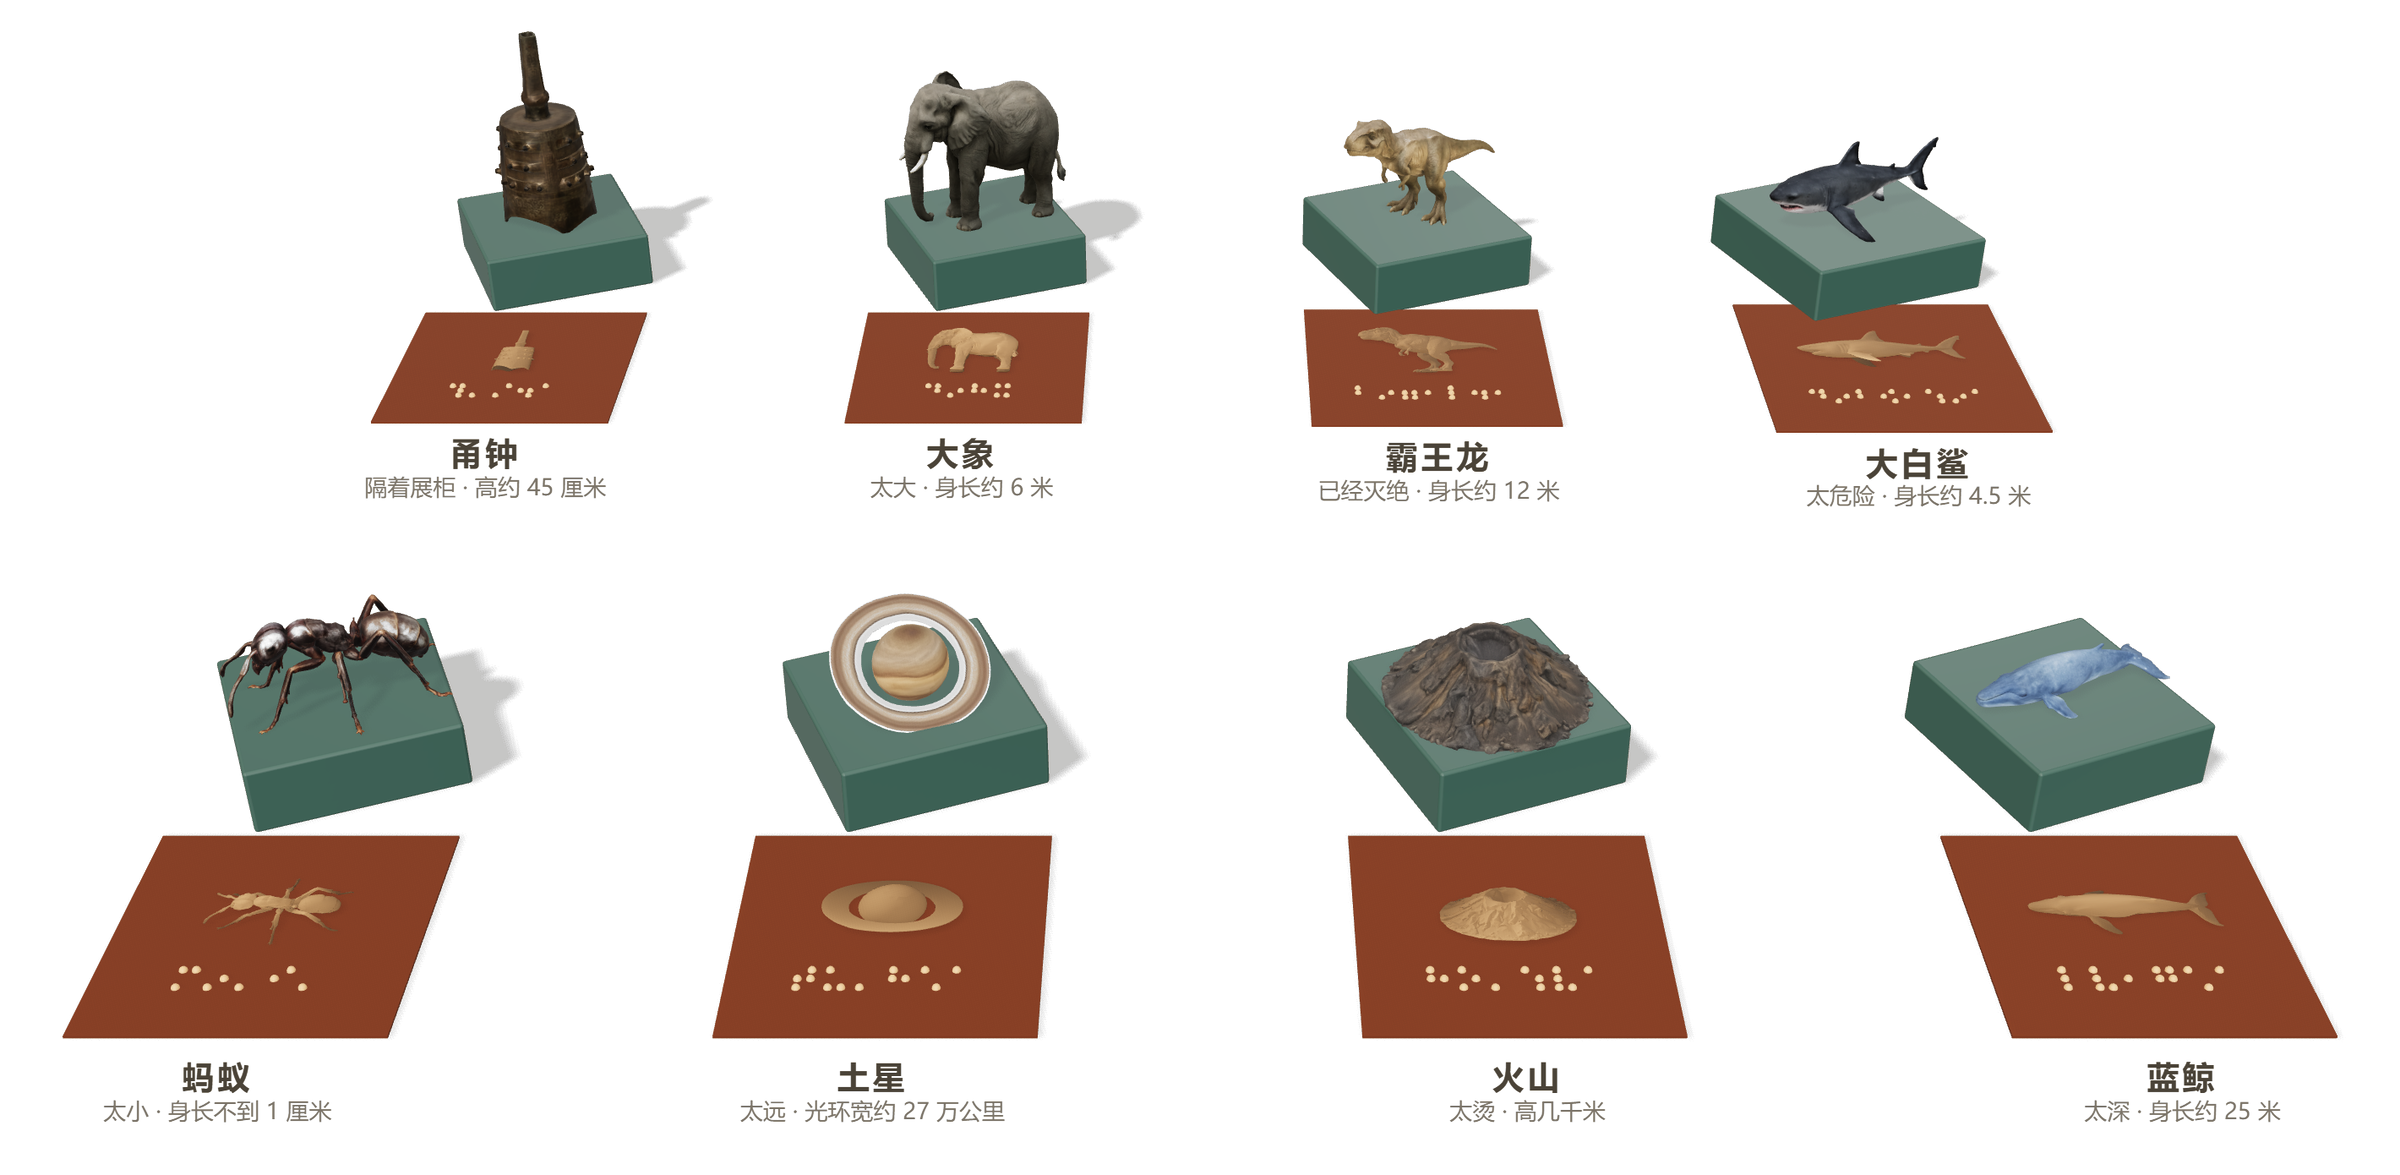
\includegraphics[width=\linewidth]{set_after.png}

\vfill
{\sffamily\color{muted}团队}\quad{\sffamily\bfseries\color{stone}\team}\par\vspace{5pt}
{\sffamily\color{muted}日期}\quad{\sffamily 2026 年 11 月 17 日}
\restoregeometry
\end{titlepage}

% =====================================================================
\section*{一页看懂}
\addcontentsline{toc}{section}{一页看懂}
\markboth{一页看懂}{}

\begin{note}[colback=white!60!cream]
\renewcommand{\arraystretch}{1.35}
\begin{tabularx}{\linewidth}{@{}>{\sffamily\bfseries\leavevmode\color{stone}}p{2.3cm}X@{}}
做了什么 & 一套给盲童的印章「万物印」。\textbf{印钮}是 Lux3D 生成的 3D 物件，孩子先用手摸，猜它是什么；\textbf{印面}在底下，刻着国家通用盲文的名字和同一物件压平的轮廓浮雕，翻过来就是答案；在印面上铺一张铜箔拓一遍，就得到一页能摸读的书，一枚一枚拓下来，孩子就有了自己做的一本书。八枚精选印收的都是孩子很难亲手摸到的东西；另有网页「造印机」：说一句话或传一张照片，几分钟后就多一枚新印。\\
怎么做 & 一句话 / 一张照片 $\to$ \textbf{Lux3D} 文生 3D / 图生 3D $\to$ GLB 模型 $\to$ 自动定朝向、转写盲文、压出浮雕 $\to$ 一枚印 $\to$ 铜箔拓片。\textbf{同一个 Lux3D 模型，立着是题目（印钮），压平是答案（印面）。}\\
为什么值得体验 & \textbf{对盲童：}太大、太远、太深、太危险、已经灭绝、隔着展柜、太小、太烫的东西，第一次能握在手里；先猜后验，答案自己就能摸到，不用等别人告诉；拓片是亲手做出来的。\newline
\textbf{对老师和家长：}孩子随口一问“长颈鹿长什么样”，不必等别人做模型，说一句话就能造一枚印（文生 3D 13 积分；现场实测从提交到新印落桌约一分半钟）。\newline
\textbf{对评委：}网页里能走完“摸—翻—拓—集”的完整流程；Lux3D 不是装饰，拿掉它，一枚印也做不出来。\\
\end{tabularx}
\end{note}

\vspace{2pt}
\begin{center}
\renewcommand{\arraystretch}{1.1}
\begin{tabularx}{\linewidth}{*{5}{>{\centering\arraybackslash}X}}
{\sffamily\bfseries\fontsize{22}{24}\selectfont\color{cinnabar}8} &
{\sffamily\bfseries\fontsize{22}{24}\selectfont\color{cinnabar}5} &
{\sffamily\bfseries\fontsize{22}{24}\selectfont\color{cinnabar}1\,{\normalsize 分}\,33\,{\normalsize 秒}} &
{\sffamily\bfseries\fontsize{22}{24}\selectfont\color{cinnabar}1\,\normalsize 积分} &
{\sffamily\bfseries\fontsize{22}{24}\selectfont\color{cinnabar}2.0\,\normalsize MB} \\
\small 枚精选印，各对应一种“摸不到” &
\small 项 Lux3D 能力用进作品 &
\small 现场实测：一句话变一枚新印（13 积分） &
\small 一张照片变一枚新印（现场约 1 分钟） &
\small 八枚印的模型，原为 67.5 MB \\
\end{tabularx}
\end{center}

\vspace{2pt}
\noindent{\sffamily\bfseries\color{stone} 评审维度速查}\par\vspace{2pt}
\noindent{\small
\renewcommand{\arraystretch}{1.25}%
\begin{tabularx}{\linewidth}{@{}>{\sffamily}p{3.6cm}X@{}}
\toprule
维度 & 在报告里看哪里 \\
\midrule
Lux3D 是核心（30\%） & 第 \ref{sec:lux} 节：每个印钮、每块印面浮雕都来自 Lux3D 模型；用到文生 3D、单图生 3D、材质重绘、四视图、多视图生 3D 五项能力；造印机现场生成（实测一句话到新印 1 分 33 秒）。\\
趣味与记忆点（25\%） & 第 \ref{sec:idea} 节：“摸—翻—拓—集”的小循环；第 \ref{sec:result} 节：动画与三联图。\\
新颖（20\%） & 第 \ref{sec:idea} 节：印章 + 盲文 + 拓印的组合；为什么拓印而不是盖章。\\
完整度（20\%） & 第 \ref{sec:process} 节：从「万物有声」转向、自我审阅、返工与前后对比；第 \ref{sec:result}、\ref{sec:blind} 节：八枚印、造印机、离线体验、无障碍细节。\\
传播（5\%） & 一句能转述的话（“这一页，是孩子自己做的。”）、演示视频、公开仓库。\\
\bottomrule
\end{tabularx}}

\vspace{4pt}
\begin{honest}
\textbf{\color{cinnabar}先说清楚：}万物印目前是\textbf{概念设计 + 可运行的数字原型}（网页、Lux3D 生成管线、渲染图、动画与视频）。我们\textbf{还没有打印实物}，也\textbf{还没有和盲童一起测试}；盲文由 liblouis 自动转写，\textbf{尚未经盲文专业人士校对}。报告里的图都是数字渲染。
\end{honest}

% =====================================================================
\section{为什么做}\label{sec:why}

\subsection{手，是盲童认识世界的窗口}
对看不见的孩子来说，认识一样东西，多半要靠手：摸到长长的鼻子，才知道大象和别的动物不一样；摸到一圈环，才明白土星为什么特别。明眼的孩子可以翻图画书、看纪录片，而对盲童来说，一张图片只是一张光滑的纸。

可课本里、故事里的很多东西，偏偏是一辈子都摸不到的：
\begin{center}
\renewcommand{\arraystretch}{1.25}
\begin{tabularx}{\linewidth}{*{4}{>{\centering\arraybackslash}X}}
\tagchip{太大} 大象 & \tagchip{太深} 蓝鲸 & \tagchip{已经灭绝} 霸王龙 & \tagchip{太危险} 大白鲨 \\
\tagchip{太小} 蚂蚁 & \tagchip{太远} 土星 & \tagchip{太烫} 火山 & \tagchip{隔着展柜} 甬钟 \\
\end{tabularx}
\end{center}
这八个词就是万物印的选题标准：\textbf{只收摸不到的东西}。

\subsection{为什么用 3D 生成，而不是实物或手工模型}
\begin{itemize}
  \item \textbf{实物带不进教室。}蓝鲸、土星、火山搬不来，馆藏文物隔着展柜，蚂蚁小到摸不出六条腿。
  \item \textbf{手工建模跟不上孩子的好奇心。}请人逐件建模、制作，费时费钱；孩子今天问长颈鹿，明天问恐龙蛋。
  \item \textbf{Lux3D 让“想摸什么就造什么”变得可行。}一句话或一张照片，几分钟、一到十几个积分，就是一个带贴图的 3D 模型。我们把这个能力接到盲文和印章上，让生成结果直接变成孩子能摸、能核对答案、能带走的东西。
\end{itemize}
因为只收摸不到的东西，“为什么非要用 3D 生成”就有了明确的答案：这些东西没有别的办法放到孩子手里。

% =====================================================================
\section{创意：万物印}\label{sec:idea}

\subsection{一枚印的三面}
\begin{figure}[H]
\centering
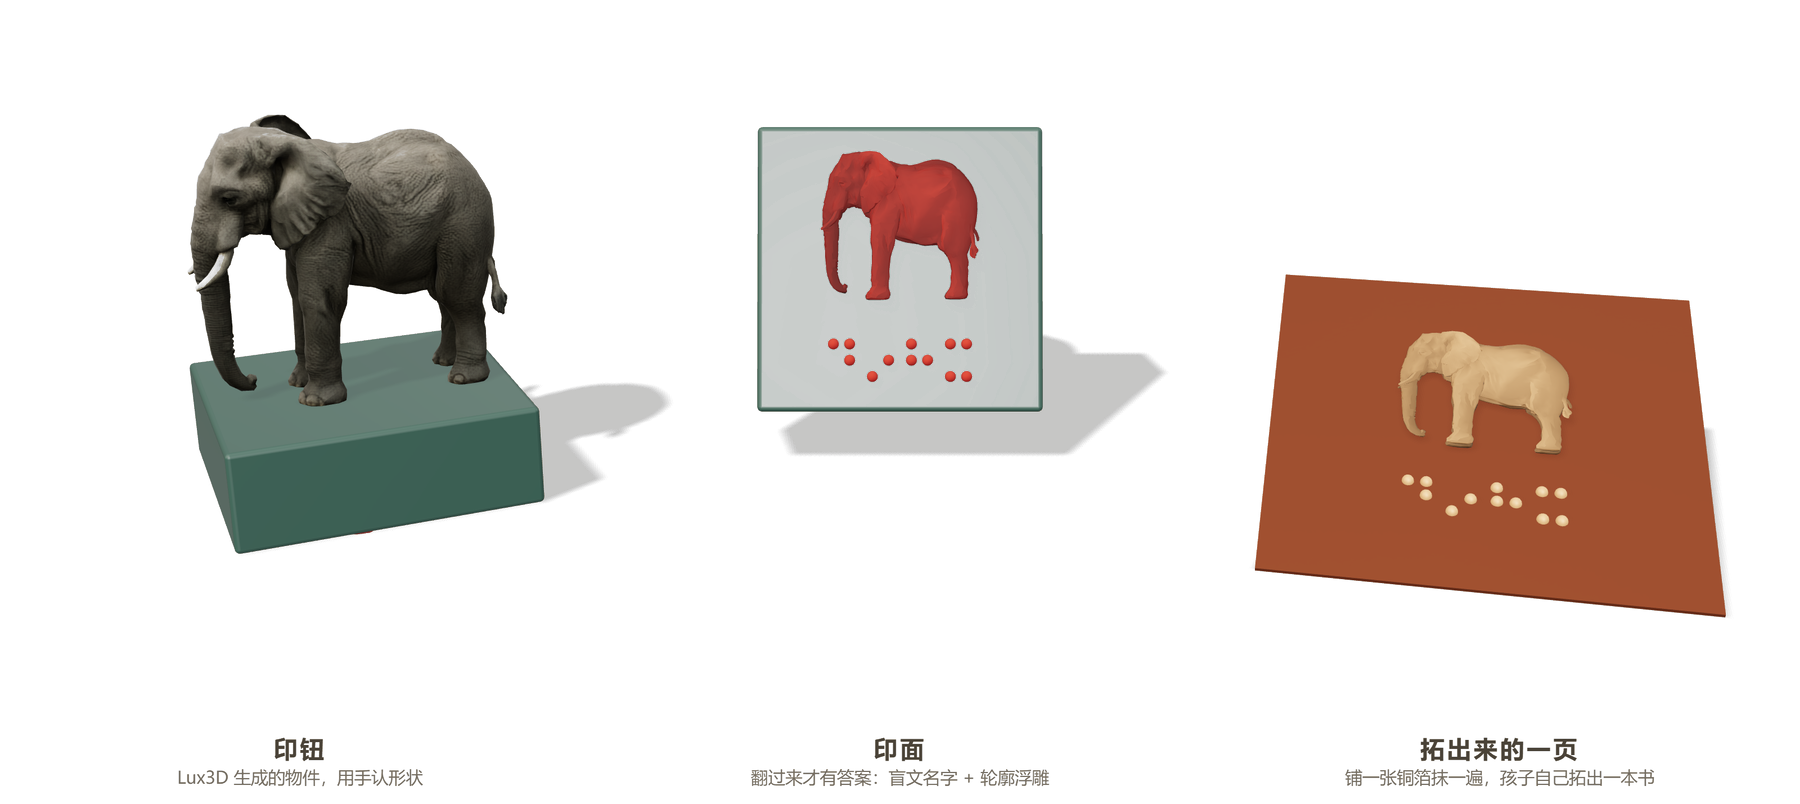
\includegraphics[width=\linewidth]{trip_elephant.png}
\caption{大象印的三联图。左：印钮，Lux3D 文生 3D 生成的非洲象（任务 6378506），用手认形状；中：印面，翻过来才有答案，上方是同一只大象压平的轮廓浮雕，下方是国家通用盲文“大象”；右：在印面上铺铜箔拓出来的一页。}
\label{fig:elephant}
\end{figure}

\subsection{玩法：摸、翻、拓、集}
\begin{figure}[H]
\centering
\begin{tikzpicture}[
  stepbox/.style={draw=stone,line width=0.8pt,fill=white!65!cream,rounded corners=4pt,
    text width=3.12cm,minimum height=2.15cm,align=flush left,inner sep=6pt,font=\small},
  num/.style={circle,fill=cinnabar,text=white,font=\sffamily\bfseries\small,inner sep=1.6pt,minimum size=17pt},
  arr/.style={-{Stealth[length=2.6mm,width=2mm]},line width=1pt,draw=stone}]
  \node[stepbox] (a) at (0,0) {{\sffamily\bfseries\color{stone}摸印钮，猜}\\[2pt]印钮上没有字。手顺着轮廓走：“摸到长鼻子了吗？”};
  \node[stepbox,right=0.62cm of a] (b) {{\sffamily\bfseries\color{stone}翻过来，验}\\[2pt]翻到印底，摸摸凸点：盲文写着名字，旁边是压平的轮廓。};
  \node[stepbox,right=0.62cm of b] (c) {{\sffamily\bfseries\color{stone}铺铜箔，拓}\\[2pt]铜箔盖在印面上抹一遍，凸起的字和图就留在箔上。};
  \node[stepbox,right=0.62cm of c] (d) {{\sffamily\bfseries\color{stone}攒成书}\\[2pt]一枚一页，攒成自己的书：“这一页，是孩子自己做的。”};
  \foreach \n/\i in {a/1,b/2,c/3,d/4} \node[num] at (\n.north west) {\i};
  \draw[arr] (a) -- (b); \draw[arr] (b) -- (c); \draw[arr] (c) -- (d);
  \draw[arr,dashed,draw=copper] (d.south) -- ++(0,-0.45) -| node[pos=0.25,below,font=\footnotesize,text=copper]{换下一枚印，再猜一次} (a.south);
\end{tikzpicture}
\caption{万物印的小循环。猜的乐趣留给孩子，答案就在同一枚印的底下，不需要明眼人在旁边揭晓。}
\label{fig:loop}
\end{figure}

\begin{itemize}
  \item \textbf{先猜后验。}印钮只给形状，不给名字。孩子先凭手感猜，再翻过来自己核对。整个过程孩子可以独立完成。
  \item \textbf{题目和答案天然一致。}印面上的浮雕就是印钮那个模型压平后的样子：手在印钮上摸到的长鼻子，翻过来还能在印面上摸到。
  \item \textbf{动手做书。}拓印是一个有声音、有手感的动作；拓完的一页可以留下来，比“听人讲一遍”更像自己的东西。
\end{itemize}

\subsection{为什么是印章，为什么拓印而不盖章}
印章天然分上下两面：上面的印钮可以是任何形状，下面的印面刚好放答案；它握在手心里大小合适，深绿印石、朱砂印面、铜箔拓片也让这套东西有自己的样子。印章和拓片都来自中国传统，但我们改了一处关键用法：\textbf{拓印，不盖章}。

\begin{figure}[H]
\centering
\begin{tikzpicture}[x=1cm,y=1cm,font=\small]
  \newcommand\sealdots[1]{\foreach \x in {#1} \fill[cinnabar] (\x-0.15,0.8) arc (180:0:0.15);}
  % (a) 印面
  \begin{scope}[shift={(0,0)}]
    \fill[stone] (0,0) rectangle (3.8,0.8);
    \sealdots{0.6,1.05,2.6}
    \fill[cinnabar] (2.95,0.8) rectangle (3.45,0.98);
    \draw[-{Stealth},muted,line width=0.7pt] (0.4,-0.32) -- (3.4,-0.32);
    \node[font=\footnotesize,text=muted] at (1.9,-0.62) {读的方向};
    \node[font=\sffamily\bfseries,text=stone] at (1.9,1.55) {印面朝上};
    \node[font=\footnotesize] at (1.9,1.2) {盲文与浮雕凸起、正向};
  \end{scope}
  % (b) 盖章
  \begin{scope}[shift={(5.4,0)}]
    \fill[clay] (0,0) rectangle (3.8,0.8);
    \foreach \x in {3.2,2.75,1.2} \fill[white] (\x+0.15,0.8) arc (0:-180:0.15);
    \fill[white] (0.35,0.62) rectangle (0.85,0.8);
    \draw[-{Stealth},muted,line width=0.7pt] (3.4,-0.32) -- (0.4,-0.32);
    \node[font=\footnotesize,text=muted] at (1.9,-0.62) {左右颠倒};
    \node[font=\sffamily\bfseries,text=cinnabar] at (1.9,1.55) {\no\ 盖在黏土上};
    \node[font=\footnotesize] at (1.9,1.2) {凹下去、镜像，摸不了};
  \end{scope}
  % (c) 拓印
  \begin{scope}[shift={(10.8,0)}]
    \fill[stone] (0,0) rectangle (3.8,0.8);
    \sealdots{0.6,1.05,2.6}
    \fill[cinnabar] (2.95,0.8) rectangle (3.45,0.98);
    \draw[copper,line width=1.7pt,line join=round] (-0.15,0.84) -- (0.42,0.84) arc (180:0:0.18) -- (0.87,0.84) arc (180:0:0.18) -- (2.42,0.84) arc (180:0:0.18) -- (2.92,0.84) -- (2.92,1.03) -- (3.48,1.03) -- (3.48,0.84) -- (3.95,0.84);
    \draw[-{Stealth},muted,line width=0.7pt] (0.4,-0.32) -- (3.4,-0.32);
    \node[font=\footnotesize,text=muted] at (1.9,-0.62) {方向不变};
    \node[font=\sffamily\bfseries,text=stone] at (1.9,1.55) {\yes\ 铺铜箔拓印};
    \node[font=\footnotesize] at (1.9,1.2) {箔上凸起、正向，可以摸读};
  \end{scope}
\end{tikzpicture}
\caption{拓印而不盖章（剖面示意）。印面上的盲文是正向凸点，翻过来就能直接摸读；如果拿它盖在黏土上，留下的是凹坑，而且左右颠倒。把铜箔铺在印面上拓，箔上得到的是凸起、正向的一页。所以印面既是答案，也是印版。}
\label{fig:rubbing}
\end{figure}

\subsection{八枚“摸不到”的印}
\begin{table}[H]
\centering
\caption{八枚精选印。盲文为 liblouis \texttt{zhcn-cbs.ctb} 转写的国家通用盲文（尚未经专业校对）；真实尺寸手写在清单 \texttt{seals.json} 里。}
\label{tab:seals}
\renewcommand{\arraystretch}{1.32}
\begin{tabularx}{\linewidth}{@{}>{\sffamily\bfseries\color{stone}}l l l l X@{}}
\toprule
\normalfont\sffamily 印 & \sffamily 盲文（国家通用盲文） & \sffamily 为什么摸不到 & \sffamily 真实尺寸 & \sffamily 印钮来源 \\
\midrule
大象   & \braille{⠙⠔⠓⠭}     & 太大     & 身长约 6 米        & 文生 3D \\
蓝鲸   & \braille{⠇⠧⠂⠛⠡⠁}   & 太深     & 身长约 25 米       & 文生 3D \\
霸王龙 & \braille{⠃⠔⠶⠂⠇⠲⠂}  & 已经灭绝 & 身长约 12 米       & 文生 3D \\
大白鲨 & \braille{⠙⠔⠃⠪⠂⠱⠔⠁} & 太危险   & 身长约 4.5 米      & 文生 3D \\
蚂蚁   & \braille{⠍⠔⠄⠊⠄}    & 太小     & 身长不到 1 厘米    & 文生 3D（返工版，见第 \ref{sec:iter} 小节） \\
土星   & \braille{⠞⠥⠄⠓⠡⠁}   & 太远     & 光环宽约 27 万公里 & 文生 3D \\
火山   & \braille{⠓⠕⠄⠱⠧⠁}   & 太烫     & 高几千米           & 文生 3D \\
甬钟   & \braille{⠹⠄⠌⠲⠁}    & 隔着展柜 & 高约 45 厘米       & 单图生 3D（大都会艺术博物馆 CC0 照片） \\
\bottomrule
\end{tabularx}
\end{table}

% =====================================================================
\section{Lux3D 是主干}\label{sec:lux}

\subsection{从一句话到一页书}
万物印的每一枚印都从 Lux3D 开始。图 \ref{fig:pipeline} 是完整管线：上排是生成，下排是造印；虚线框里的步骤由造印机后端自动完成，不需要手工建模。

\begin{figure}[tbp]
\centering
\begin{tikzpicture}[
  font=\small,
  box/.style={draw=rule,line width=0.7pt,fill=white!65!cream,rounded corners=3pt,align=flush center,inner sep=5pt},
  arr/.style={-{Stealth[length=2.6mm,width=2mm]},line width=1pt,draw=stone}]
  % 上排
  \node[box,text width=2.7cm] (txt) at (0,0.85) {{\sffamily\bfseries 说一句话}\\{\footnotesize “我想摸摸长颈鹿”}};
  \node[box,text width=2.7cm] (img) at (0,-0.85) {{\sffamily\bfseries 带一张照片}\\{\footnotesize 玩具、馆藏、插图}};
  \node[draw=cinnabar,line width=1.3pt,fill=white,rounded corners=4pt,inner sep=6pt,align=flush left,text width=6.1cm] (lux) at (5.6,0) {%
    {\sffamily\bfseries\large\color{cinnabar}Aholo Lux3D}\hfill{\footnotesize\color{muted}每一枚印的来源}\\[3pt]
    {\footnotesize\renewcommand{\arraystretch}{1.12}%
    \begin{tabular}{@{}l@{\hspace{8pt}}l@{}}
      文生 3D（G1-Turbo） & 13 积分 · 1.5--4 分钟\\
      单图生 3D & 1 积分 · 约 1 分钟\\
      材质重绘 & 7 积分 / 版\\
      单图四视图 $\to$ 多视图生 3D & 24 + 1 积分
    \end{tabular}}};
  \node[box,text width=2.75cm] (glb) at (11.75,0) {{\sffamily\bfseries GLB 模型}\\{\footnotesize 形状 + PBR 贴图\\大致是真实尺度}};
  \draw[arr] (txt.east) -- (txt.east -| lux.west);
  \draw[arr] (img.east) -- (img.east -| lux.west);
  \draw[arr] (lux) -- (glb);
  % 下排
  \node[box,text width=4.3cm,align=flush left] (make) at (11.0,-3.55) {{\sffamily\bfseries 自动造印}\\[1pt]{\footnotesize
    \textcolor{cinnabar}{①} 朝向：俯视主轴 $\to$ 侧身朝外\\
    \textcolor{cinnabar}{②} 盲文：liblouis 国家通用盲文\\
    \textcolor{cinnabar}{③} 浮雕：按投影角把模型压平\\
    \textcolor{cinnabar}{④} 合成：印钮 + 印身 + 印面}};
  \node[box,text width=3.9cm] (seal) at (5.3,-3.55) {{\sffamily\bfseries 一枚印}\\[1pt]{\footnotesize 印钮 = 原模型：用手猜\\印面 = 浮雕 + 盲文：答案}};
  \node[box,text width=2.7cm] (rub) at (0,-3.55) {{\sffamily\bfseries 铜箔拓片}\\{\footnotesize 一枚一页\\攒成自己的书}};
  \draw[arr] (glb.south) -- (glb.south |- make.north) node[midway,right,font=\footnotesize,text=muted]{下载 · 校验};
  \draw[arr] (make) -- (seal);
  \draw[arr] (seal) -- (rub);
  \node[font=\kai\small,text=cinnabar] at (5.6,-1.78) {同一个 Lux3D 模型：立着是题目，压平是答案};
  \begin{scope}[on background layer]
    \node[draw=stone,dashed,line width=0.6pt,rounded corners=5pt,inner sep=7pt,fit=(make)(seal)] (svc) {};
  \end{scope}
  \node[anchor=north east,font=\scriptsize\sffamily,text=stone] at ([yshift=-2pt]svc.south east) {造印机后端：排队（最多 5 个并发）· 先报价再生成 · 每日预算 · 断点恢复};
\end{tikzpicture}
\caption{万物印的生成管线。印钮、印面浮雕、三种印材、甬钟的照片重建，都来自 Lux3D 的生成结果；我们写的代码负责把模型变成“印”：定朝向、转写盲文、压浮雕、拼合、出图。}
\label{fig:pipeline}
\end{figure}

\textbf{拿掉 Lux3D 会怎样？}印钮没有了，印面浮雕也没有了：浮雕就是把同一个模型按选定的角度压平得到的。造印机也就只剩一个空壳。Lux3D 在这里不是给成品加一层“AI 味”，而是每一枚印的原料。

\subsection{用到的五项 Lux3D 能力}
\begin{table}[H]
\centering
\caption{万物印用到的 Lux3D 能力。积分取自各任务实际报价。时间为实测范围：较短的数字来自 11 月 17 日现场录制（从提交计到新印落桌，见表 \ref{tab:live}），较长的来自早期生成记录。}
\label{tab:lux}
\renewcommand{\arraystretch}{1.3}
\noindent{\small
\begin{tabularx}{\linewidth}{@{}>{\sffamily\bfseries\leavevmode\color{stone}}p{2.35cm}X>{\raggedright\arraybackslash}p{2.5cm}>{\raggedright\arraybackslash}p{2.75cm}@{}}
\toprule
\normalfont\sffamily 能力 & \sffamily 在万物印里做什么 & \sffamily 实测成本 & \sffamily 任务号 \\
\midrule
文生 3D & 七枚印钮（大象、蓝鲸、霸王龙、大白鲨、蚂蚁、土星、火山）；造印机“说一句话” & 13 积分，1.5--4 分钟 & 如大象 6378506 \\
单图生 3D & 甬钟印钮，输入是一张大都会艺术博物馆 CC0 照片；造印机“带一张照片” & 1 积分，约 1 分钟 & 4523886 \\
材质重绘 & 同一枚大象印换上青铜、玄武岩、木雕三种印材；几何不变，盲文和朝向直接沿用 & 每版 7 积分 & 6447867 / 6447866 / 6447868 \\
单图四视图 & 从一张馆藏甬钟照片补出四个角度 & 24 积分 & 4527847 \\
多视图生 3D & 用这四张图重建一枚甬钟，作为对照示例 & 1 积分 & 4527961 \\
\bottomrule
\end{tabularx}}
\end{table}

八枚精选印的输入都记录在生成目录的 \texttt{task.json} 里，可以追溯。文生 3D 统一用 G1-Turbo、开启 PBR、目标约一万面：

\noindent{\small
\renewcommand{\arraystretch}{1.22}%
\begin{tabularx}{\linewidth}{@{}>{\sffamily\bfseries\color{stone}}l X r@{}}
\toprule
\normalfont\sffamily 印 & \sffamily Lux3D 输入（提示词或照片） & \sffamily 任务号 \\
\midrule
大象 & 「一只站立的非洲象，写实风格，完整全身，四脚着地，白色背景」 & 6378506 \\
蓝鲸 & 「一头蓝鲸，写实风格，完整全身，身体舒展，白色背景」 & 6380049 \\
霸王龙 & 「一只站立的霸王龙，写实风格，完整全身，白色背景」 & 6380057 \\
大白鲨 & 「一条大白鲨，写实风格，完整全身，白色背景」 & 6380066 \\
土星 & 「土星，带完整的行星环，写实风格，白色背景」 & 6380083 \\
火山 & 「一座火山，圆锥形山体完整，顶部有火山口，写实风格，白色背景」 & 6380377 \\
蚂蚁 & 返工版提示词见第 \ref{sec:iter} 小节 & 6446180 \\
甬钟 & 大都会艺术博物馆开放获取照片 DP154556（战国青铜甬钟，CC0） & 4523886 \\
\bottomrule
\end{tabularx}}

\subsection{一张馆藏照片 \texorpdfstring{$\to$}{→} 一枚甬钟印}
甬钟是“隔着展柜”的代表。我们没有给它写提示词，而是直接把博物馆公开的一张照片交给 Lux3D 单图生 3D：1 积分、不到 1 分钟，就得到带青铜贴图的模型，印钮上的长柄、钟体和下缘凹口都在。

\begin{figure}[H]
\centering
\begin{tikzpicture}
  \node[inner sep=0,draw=rule,line width=0.5pt] (p) {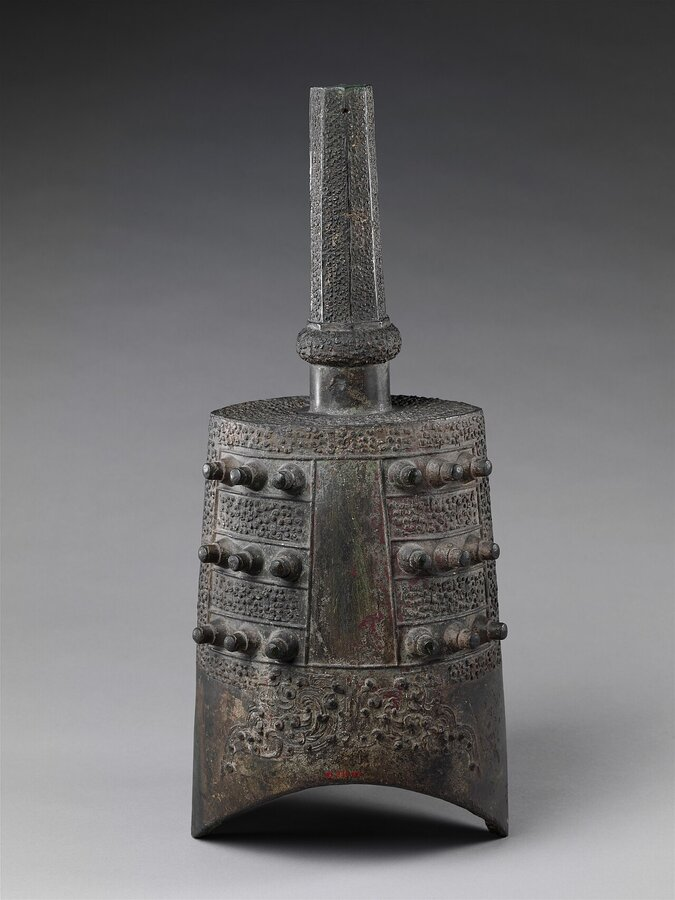
\includegraphics[height=4.6cm]{met_DP154556.jpg}};
  \node[inner sep=0,draw=rule,line width=0.5pt,right=1.5cm of p] (s) {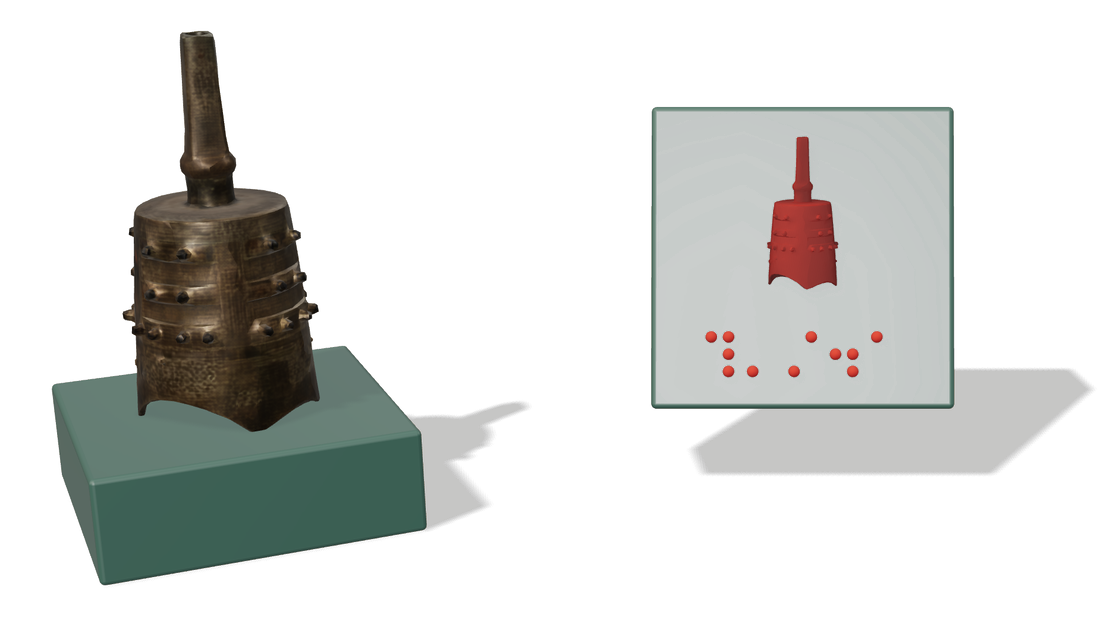
\includegraphics[height=4.6cm]{yongzhong_knobface.png}};
  \draw[-{Stealth[length=3mm,width=2.4mm]},line width=1.3pt,draw=cinnabar] (p.east) -- (s.west)
    node[midway,above,font=\footnotesize\sffamily,text=cinnabar,align=flush center]{Lux3D\\单图生 3D}
    node[midway,below,font=\scriptsize,text=muted,align=flush center]{1 积分\\不到 1 分钟};
\end{tikzpicture}

\vspace{4pt}
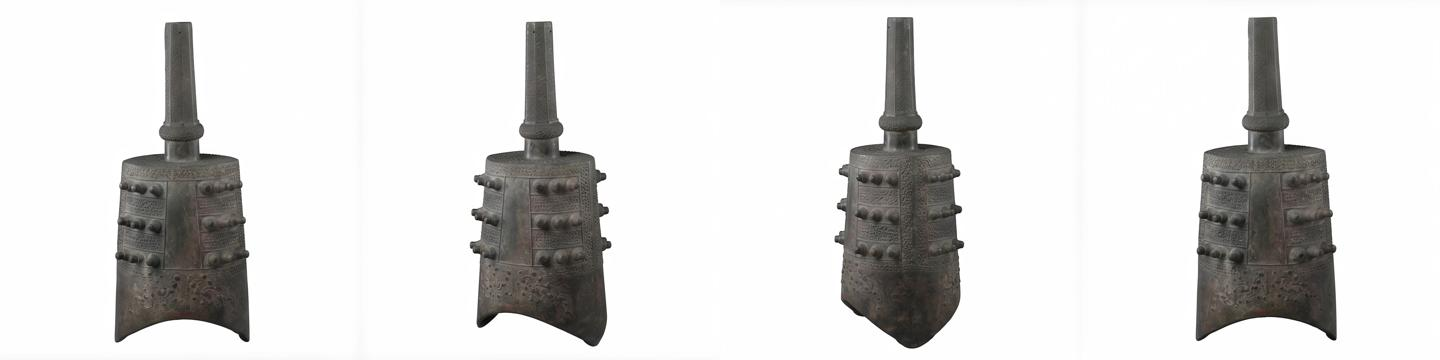
\includegraphics[width=\linewidth]{yongzhong_views.jpg}
\caption{上：大都会艺术博物馆开放获取照片 DP154556（CC0），经 Lux3D 单图生 3D 变成甬钟印的印钮与印面。下：用同一张照片调用 Lux3D 单图四视图（24 积分）补出的四个角度，再用多视图生 3D（1 积分）重建。补出的角度是生成结果，不是真实拍摄。}
\label{fig:yongzhong}
\end{figure}

四视图让我们能从一张照片“绕到背后”去看。我们也如实记录了它的边界：四视图本身显示钟体截面的宽深比约 0.85，重建后的模型却是 0.95，棱角被抹圆了一些。所以造印机里的照片上传仍走单图生 3D，四视图重建作为示例保留在工作台里。

\subsection{材质重绘：同一枚印，三种印材}
\begin{figure}[H]
\centering
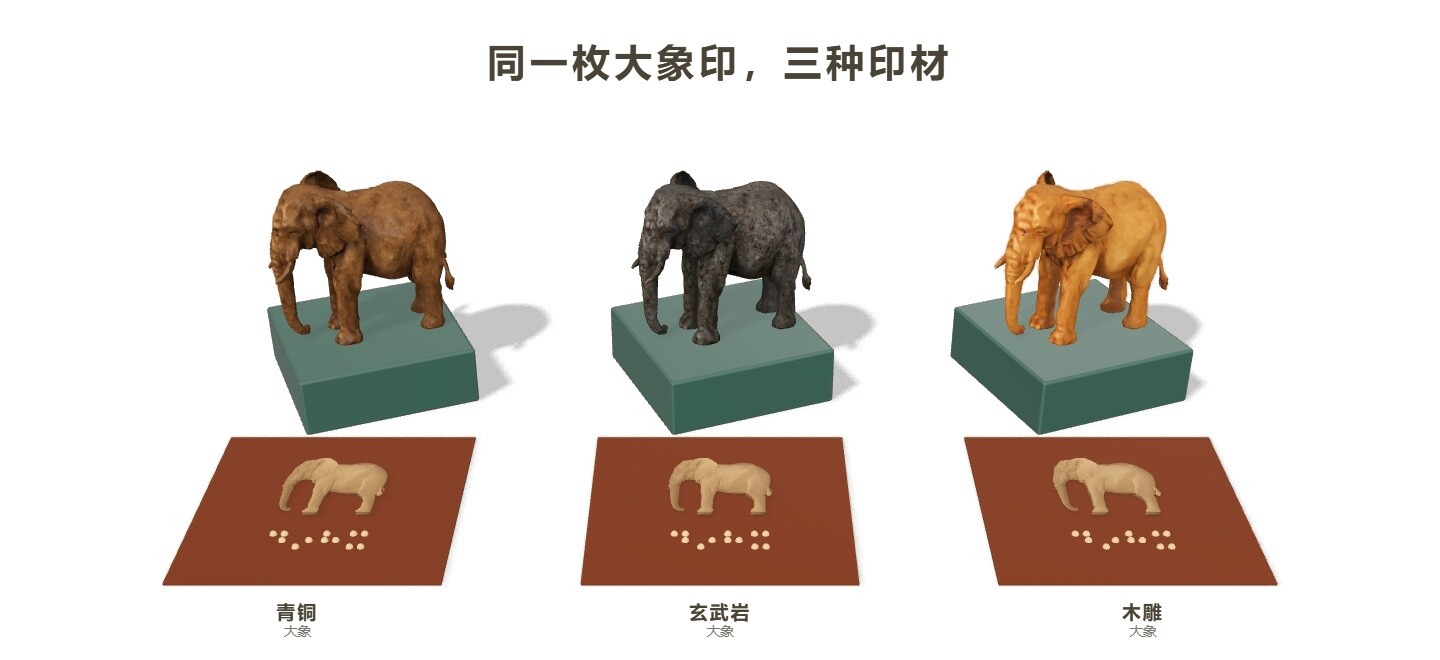
\includegraphics[width=0.92\linewidth]{elephant_materials.jpg}
\caption{同一枚大象印经 Lux3D 材质重绘换上青铜、玄武岩、木雕三种外观（任务 6447867、6447866、6447868，每版 7 积分）。三版与原模型都是 7{,}487 个顶点、9{,}556 个三角面，位置与索引逐项相同，所以盲文、朝向和印面浮雕都能直接沿用。}
\label{fig:materials}
\end{figure}

印钮换材质，对盲童的手来说形状不变；对一起玩的明眼伙伴和老师来说，同一个形状有了“青铜器”“石雕”“木雕”的样子，也为将来按材质打印或配上敲击声音（见第 \ref{sec:next} 节）留了接口。

\subsection{造印机：现场造一枚新印}
造印机是一个网页工作台（\texttt{maker.html}）。孩子或老师说一句话、或者上传一张照片，后端调用 Lux3D 生成模型，自动算盲文和朝向，一两分钟后新印就出现在工作台上（现场实测见表 \ref{tab:live}），可以马上翻面、拓印、放进“我的印集”。

\begin{figure}[H]
\centering
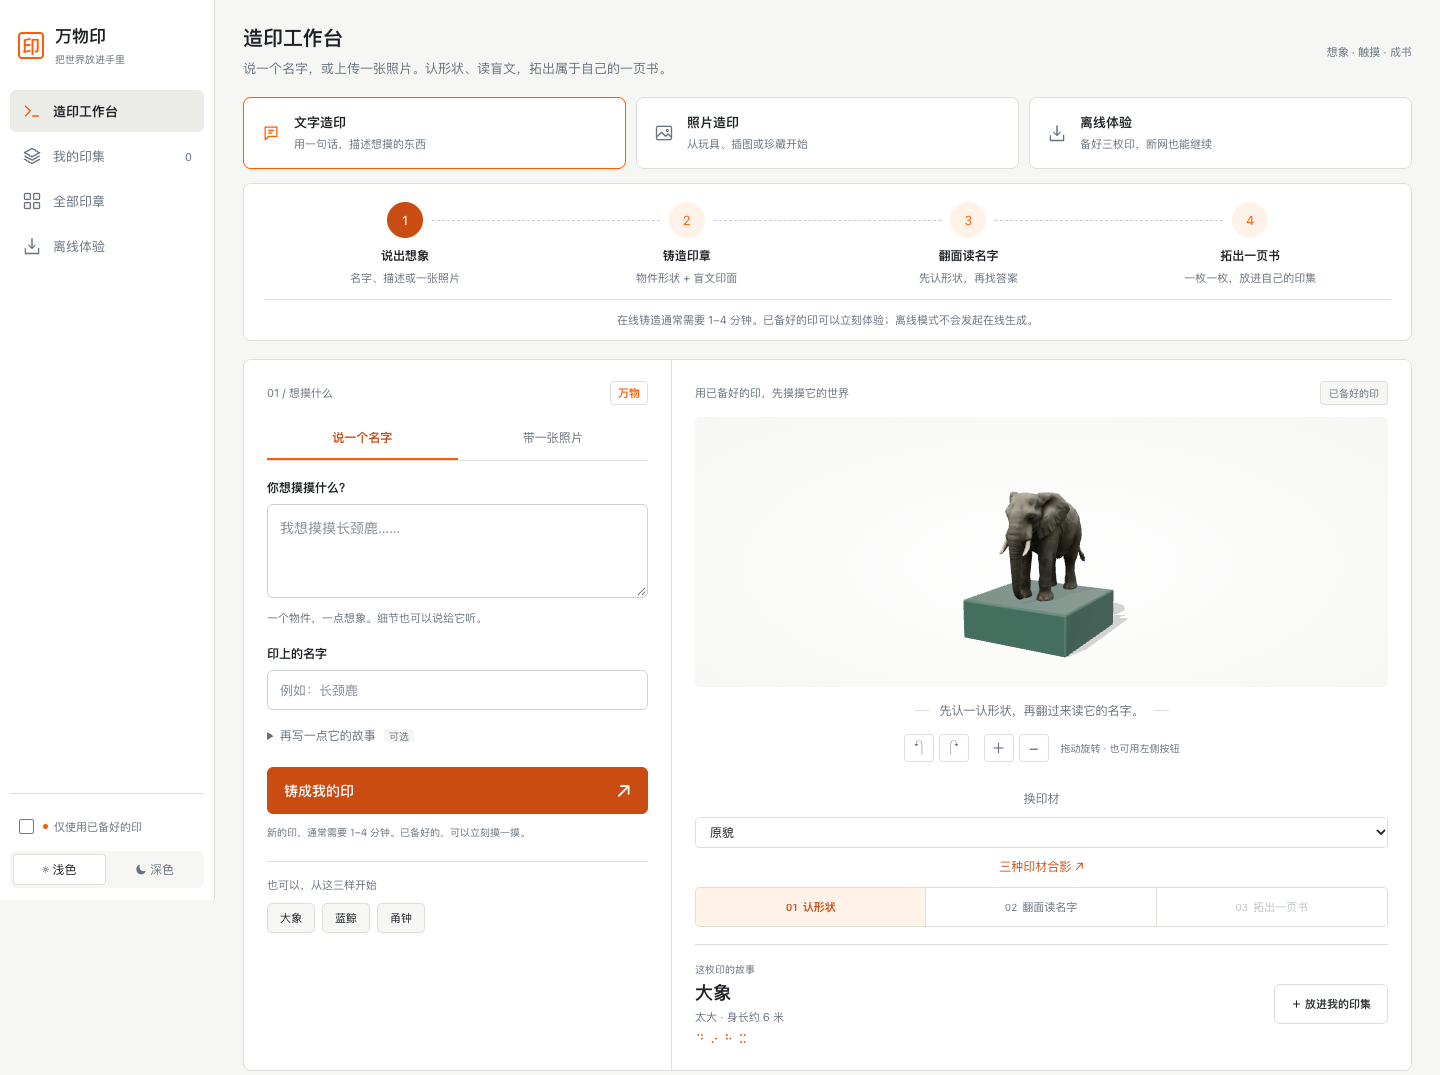
\includegraphics[width=0.94\linewidth]{maker.png}
\caption{造印工作台。左栏是“说一个名字 / 带一张照片”两种入口，右侧舞台可以拖动查看印钮、翻面读名字、拓出一页，下方是“我的印集”和离线体验。截图中展示的是已备好的大象印。}
\label{fig:maker}
\end{figure}

\begin{figure}[H]
\centering
\begin{tikzpicture}[
  st/.style={draw=stone,line width=0.7pt,fill=white!65!cream,rounded corners=8pt,font=\footnotesize\sffamily,inner xsep=7pt,inner ysep=4pt,align=flush center},
  arr/.style={-{Stealth[length=2mm]},line width=0.8pt,draw=stone}]
  \node[st] (q) {排队\\queued};
  \node[st,right=0.55cm of q] (p) {报价\\quoting};
  \node[st,right=0.55cm of p] (g) {生成\\generating};
  \node[st,right=0.55cm of g] (d) {下载\\downloading};
  \node[st,right=0.55cm of d,fill=stone,text=white] (c) {完成\\completed};
  \node[st,below=0.42cm of g,draw=cinnabar,text=cinnabar] (f) {失败（给出中文原因）\\failed};
  \draw[arr] (q)--(p); \draw[arr] (p)--(g); \draw[arr] (g)--(d); \draw[arr] (d)--(c);
  \draw[arr,draw=cinnabar,dashed] (p.south) |- (f.west);
  \draw[arr,draw=cinnabar,dashed] (d.south) |- (f.east);
\end{tikzpicture}
\caption{一枚新印在造印机后端的状态。页面显示当前状态和已等待时间；预计时间（文生约 240 秒、图生约 60 秒）只作参考，不显示虚构的进度百分比。}
\label{fig:states}
\end{figure}

\begin{table}[H]
\centering
\caption{造印机现场实测：2026 年 11 月 17 日录制演示视频时，本机后端调用 Lux3D API 的两次完整运行。时间为界面计时，从点击“铸成我的印”到新印落在桌上。}
\label{tab:live}
\renewcommand{\arraystretch}{1.35}
{\small
\begin{tabularx}{\linewidth}{@{}>{\raggedright\arraybackslash}X l l l l@{}}
\toprule
\sffamily 输入 & \sffamily Lux3D 能力 & \sffamily 提交 $\to$ 落桌 & \sffamily 积分 & \sffamily 自动转写的盲文 \\
\midrule
一句话“我想摸摸长颈鹿” & 文生 3D & 1 分 33 秒 / 1 分 37 秒 & 每次 13 & 长颈鹿\ \braille{⠟⠦⠛⠡⠄⠇⠥} \\
大都会艺术博物馆 CC0 青铜钟照片（DP155212，春秋） & 单图生 3D & 约 63--68 秒 & 每次 1 & 青铜钟\ \braille{⠅⠡⠁⠞⠲⠌⠲⠁} \\
\bottomrule
\end{tabularx}}
\end{table}

两次录制共花 28 积分（每次 13 + 1）。盲文名字和俯视朝向都由后端自动算出，模型没有经过任何人工修改；两枚新印随后出现在视频结尾的十枚合影里。

后端（\texttt{pipeline/scripts/serve\_seals.py}）为了“现场演示不出事”做了这些事：
\begin{itemize}
  \item \textbf{先报价，再生成。}单次上限文生 15、图生 3 积分，另有按北京时间计的每日预算；超过上限就不创建任务。
  \item \textbf{最多 5 个并发。}这是 Lux3D 的并发上限；第 6 个起进入 SQLite 持久队列，不会被拒。
  \item \textbf{断线、刷新、重启都能接着来。}同一次点击带同一个幂等键，不会重复扣费；进程重启后，已知任务号的继续轮询下载，排队的继续执行。
  \item \textbf{密钥只在后端。}Lux3D 密钥从不进入前端，响应里也不带上游下载地址。
\end{itemize}

同一套流程也能用两条命令走完，这是我们添加新印的日常做法：
\begin{note}[colback=white]
\begin{Verbatim}[fontsize=\footnotesize,commandchars=\\\{\},formatcom=\xeCJKsetup{CJKecglue={\hspace{0pt}}}]
\textcolor{muted}{# 1) 一句话 -> Lux3D 文生 3D（先报价，超过上限不建任务）}
python scripts/lux3d_generate.py --prompt "一只站立的长颈鹿，写实风格，完整全身，白色背景" \textbackslash
    --max-credits 15 --out out/lux3d/giraffe
\textcolor{muted}{# 2) 模型 -> 盲文 + 朝向 -> 写进印的清单 seals.json}
python scripts/seal_meta.py out/lux3d/giraffe/output_0.glb --label 长颈鹿 \textbackslash
    --into ../web/public/seals.json --name giraffe --why 太高 --real "高约 5 米"
\end{Verbatim}
\end{note}

\subsection{Lux3D 的脾气，怎样影响了设计}
\begin{itemize}
  \item \textbf{提示词要写“写实风格，完整全身，白色背景”}，避免生成背景和底座；细长部件要写清数量和朝向（蚂蚁就是教训，见第 \ref{sec:iter} 小节）。
  \item \textbf{尺度大致是真实米制，但不可靠}：蓝鲸约 25 米、蚂蚁约 1 厘米，霸王龙却只有 0.5 米。所以网页把模型统一缩放到印身大小，标签上的真实尺寸由我们手写。
  \item \textbf{俯视主轴决定朝向}：对模型表面采样 20 万点，求俯视平面上的主轴，让动物侧身朝外；俯视接近圆的（钟、星球、火山，长短轴比小于 1.12）保持原样。
  \item \textbf{生成的 GLB 每个 7--10 MB}：上网页前用 meshopt 压缩几何、贴图转 1024 像素 WebP，八枚印共 67.5 MB 降到约 2.0 MB（见第 \ref{sec:process} 节）。
\end{itemize}

% =====================================================================
\section{过程与迭代}\label{sec:process}

\subsection{时间线}
\begin{figure}[H]
\centering
\begin{tikzpicture}[x=1cm,y=1cm]
  \newcommand\ev[5]{% y, 日期, 标题, 说明, 颜色
    \fill[#5] (0,#1) circle (4.5pt);
    \node[anchor=east,font=\sffamily\bfseries\small,text=#5] at (-0.35,#1) {#2};
    \node[anchor=north west,text width=13.4cm,inner sep=0pt,font=\small,align=flush left] at (0.42,#1+0.19) {{\sffamily\bfseries\color{stone}#3}\quad #4};}
  \draw[rule,line width=1.4pt] (0,0.35) -- (0,-7.45);
  \ev{0}{10/31}{「万物有声」方案与原型}{Lux3D 材质 $\to$ 体素有限元算振动 $\to$ 声音；做了叩物沙盒、编钟架、听触页和带盲文底座的触摸件。}{muted}
  \ev{-1.2}{11/11}{转向「万物印」}{听觉做主线不好讲清楚，打印件也还原不了材质；改做给盲童认识世界的印章，Lux3D 生成首批八枚。}{cinnabar}
  \ev{-2.4}{11/11}{造印机}{后端：持久队列、最多 5 个并发、每日预算、幂等重试、断点恢复；工作台：文字 / 照片造印、翻面拓印、收藏、离线体验。}{stone}
  \ev{-3.6}{11/11}{自我审阅}{逐枚对照三联图、合影和概念片，再从原始 GLB 出三向图：保留七枚，返工蚂蚁，改蓝鲸、土星、火山的印面投影，改字幕措辞。}{stone}
  \ev{-4.8}{11/11}{返工}{新工蚁（任务 6446180，一次成功）；可读浮雕与铜箔观感；三种印材（材质重绘）；四视图与多视图重建。}{stone}
  \ev{-6.0}{11/13}{合入主干，模型瘦身}{各分支经评审合入；八枚印的模型 67.5 MB $\to$ 约 2.0 MB。}{stone}
  \ev{-7.2}{11/17}{现场铸印，提交}{录制演示视频时用造印机现场调用 Lux3D，铸出长颈鹿（文生）和青铜钟（图生）两枚新印；提交视频与这份报告书。}{cinnabar}
\end{tikzpicture}
\caption{项目时间线（日期据方案文档与 git 提交记录）。}
\label{fig:timeline}
\end{figure}

\subsection{起点：「万物有声」，以及为什么放下它}
最早的方向叫「万物有声」：Lux3D 给了物体外观，我们给它一副会振动的身体。程序从 Lux3D 的 PBR 贴图推断材质，用体素有限元算出模态，再合成敲击声；同一件物体按音高缩放，就能排成编钟架演奏一段曲子。

\begin{figure}[H]
\centering
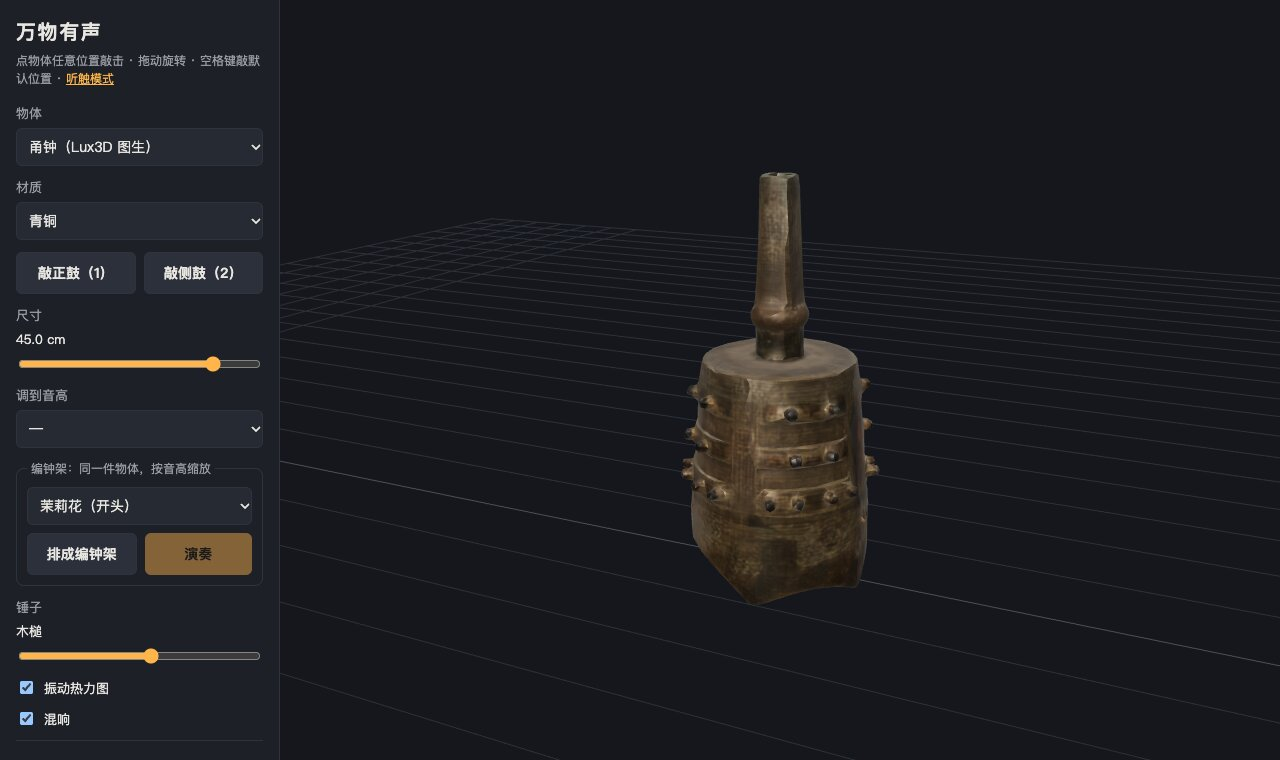
\includegraphics[width=0.49\linewidth]{wwys_strike.jpg}\hfill
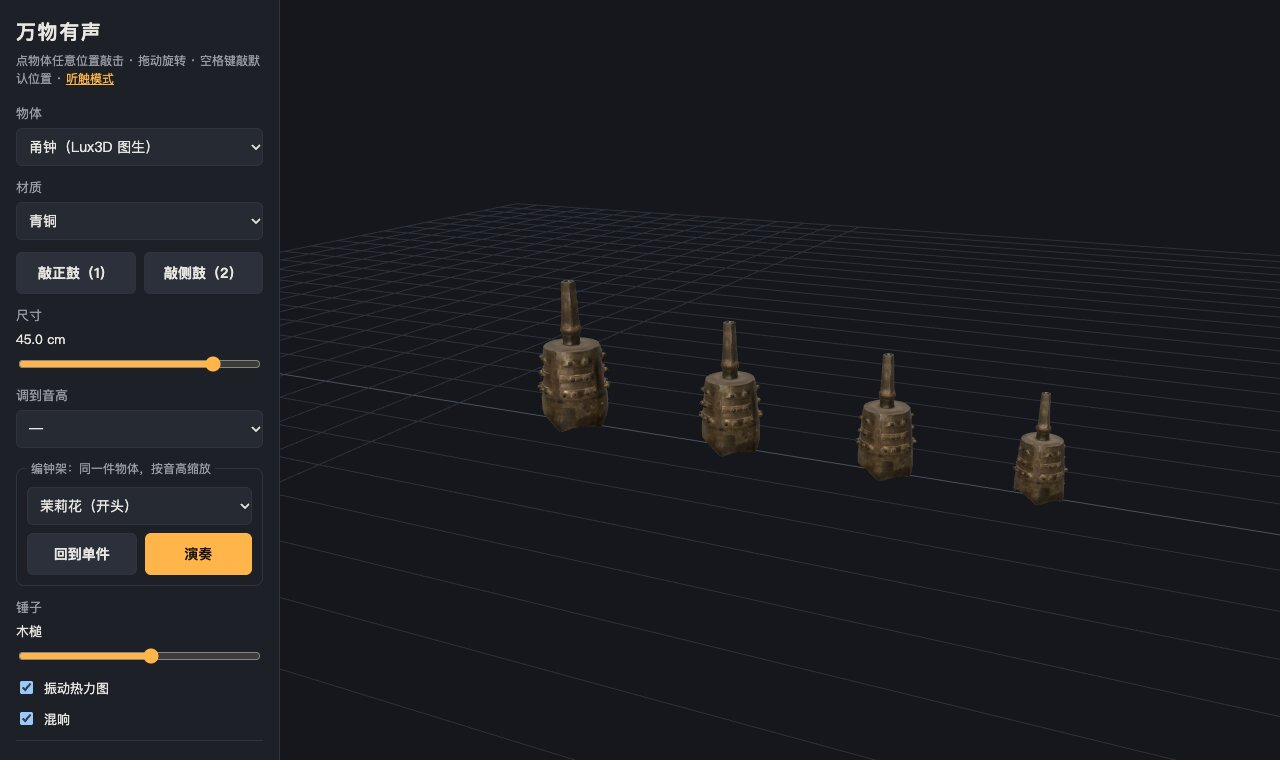
\includegraphics[width=0.49\linewidth]{wwys_rack.jpg}
\caption{10 月 31 日的「万物有声」原型。左：叩物沙盒里 Lux3D 图生的甬钟，可以分别敲正鼓和侧鼓；右：同一件甬钟按音高缩放成编钟架。}
\label{fig:wwys}
\end{figure}

11 月 11 日我们放下了它作为主线，原因有两个：一是以听觉为主的玩法很难一句话讲清楚；二是打印出来的触摸件只能还原形状，还原不了材质，“摸起来全是塑料”。但其中两样东西留了下来：\textbf{给视障孩子做东西}的初心，和\textbf{带国家通用盲文底座的触摸件}代码。它们长成了万物印；声音降为彩蛋和扩展方向。

\subsection{审阅：先挑自己的毛病}
八枚印生成出来以后，我们没有急着往下做，而是逐枚对照三联图、合影和 38.9 秒概念片的逐秒取帧。为了分清“模型本身有问题”还是“压平的角度有问题”，我们直接从原始 GLB 出了俯视、底视、斜视三向图（图 \ref{fig:review}）。

\begin{figure}[H]
\centering
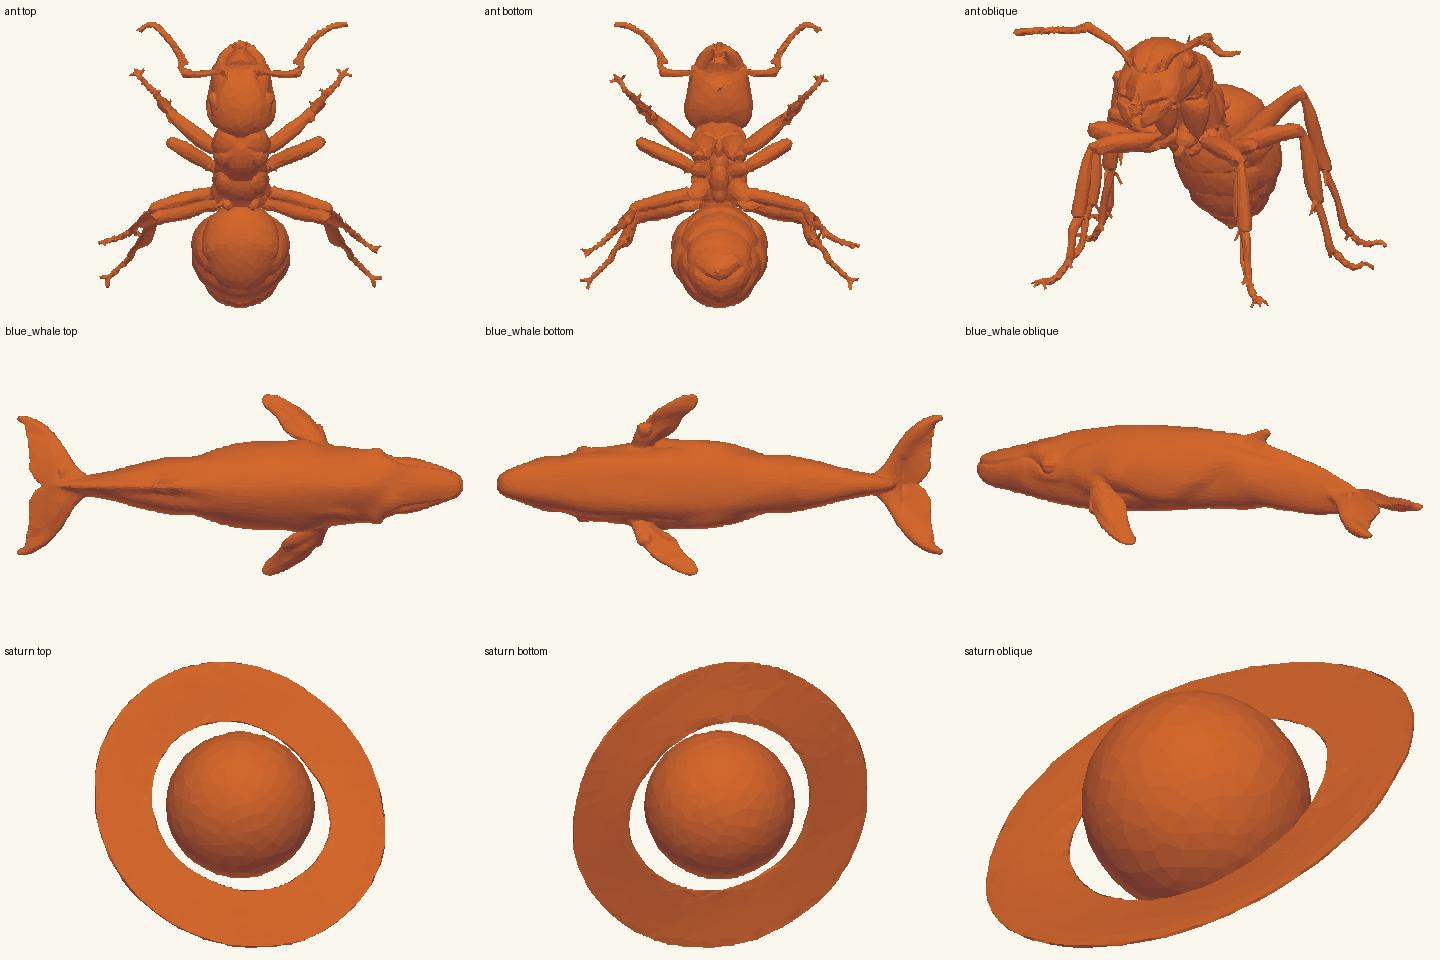
\includegraphics[width=0.86\linewidth]{review_angles.jpg}
\caption{审阅时从原始 GLB 直接出的三向几何图（统一底色只为看轮廓）。蓝鲸俯视有左右胸鳍和展开的双叶尾鳍、土星俯视有闭合的环和环内空隙：问题在印面投影，不在模型。第一版蚂蚁的细足贴叠、分叉，不适合教孩子数六条腿：问题在模型。}
\label{fig:review}
\end{figure}

审阅的结论是：\textbf{保留七枚，返工蚂蚁一枚}；蓝鲸、土星、火山保留印钮，只改它们在印面上的投影；字幕措辞也一起改，例如“已消失”改为“已经灭绝”，甬钟的“太珍贵”改为“隔着展柜”，“翻过来，答案在底下”改为能照着做的“翻到印底，摸摸凸点”。

\subsection{迭代对比}\label{sec:iter}
以下“改前”取自首批渲染（git 提交 \texttt{816c16f}），“改后”是现在的版本（\texttt{3c22a8b} 与 \texttt{3d3f610}）。

\begin{figure}[H]
\centering
\beforeafter{ant_before.png}{ant_after.png}{改前：第一版蚂蚁}{改后：重新生成的工蚁}
\caption{\textbf{蚂蚁：重新生成模型。}第一版提示词是「一只蚂蚁，写实风格，完整全身，六条腿和触角清晰，白色背景」，生成的蚂蚁细足贴叠，侧面印纹很难从胸部逐条追到足尖。返工提示词写清了结构：「单只写实工蚁，头胸腹分明、细腰；三对足均从胸部长出，前足向前、中足向两侧、后足向后，六个足尖彼此分开；头部两根弯折触角，完整全身，白底，无底座。」Lux3D 任务 6446180 一次成功（13 积分），印面改用俯视投影，六条腿和两根触角都能数清。}
\label{fig:ant}
\end{figure}

\begin{figure}[H]
\centering
\beforeafter{saturn_before.png}{saturn_after.png}{改前}{改后}
\caption{\textbf{土星：只改印面投影。}改前从正侧面压平，印面像一个圆球坐在弯托上，拓片也丢了环孔。改后把投影抬高约 10°（0.18 弧度），球的左右两侧各露出一块环内空隙，手能摸出“球外套着一个环”。}
\label{fig:saturn}
\end{figure}

\begin{figure}[H]
\centering
\beforeafter{blue_whale_before.png}{blue_whale_after.png}{改前}{改后}
\caption{\textbf{蓝鲸：改为斜俯视。}改前是侧面剪影，拓片像一根细梭。改后用约 73°（1.27 弧度）的斜俯视压平，左右胸鳍和双叶尾鳍与躯干分开，鲸的身形一摸就和鲨鱼不一样。}
\label{fig:whale}
\end{figure}

\begin{figure}[H]
\centering
\beforeafter{volcano_before.png}{volcano_after.png}{改前}{改后}
\caption{\textbf{火山：带一点俯角。}改前的侧影像一座普通山丘。改后用约 37°（0.65 弧度）的俯角压平，山坡的沟壑和顶上的火山口同时出现在印面上，这才是“火山”而不是“山”。}
\label{fig:volcano}
\end{figure}

\begin{figure}[H]
\centering
\beforeafter{set_before.png}{set_after_small.png}{改前}{改后}
\caption{\textbf{整套合影。}除上面四处外，铜箔拓片压低了正面高光、加了掠射光，并让浮雕越高处越亮（像被抹亮的铜），点阵不再和底色混成一片；标签措辞改为“已经灭绝”“隔着展柜”。}
\label{fig:set}
\end{figure}

这些改动有一个共同原则：\textbf{不只转相机}。整台相机换个角度，并不能恢复压扁时已经消失的轮廓；必须为每一枚印单独选“压平的角度”，让孩子用手能区分的特征（环孔、尾鳍、六条腿、火山口）在印面上留下来。

\subsection{瘦身：让网页打开得动}
Lux3D 生成的 GLB 每个 7--10 MB。我们用 meshopt 压缩几何、把贴图缩到 1024 像素并转 WebP，网页统一用带 meshopt 解码的加载器读取：

\noindent{\small
\renewcommand{\arraystretch}{1.25}%
\setlength{\tabcolsep}{4.2pt}%
\begin{tabularx}{\linewidth}{@{}>{\sffamily}l*{8}{>{\centering\arraybackslash}X}>{\centering\arraybackslash\bfseries}X@{}}
\toprule
 & 大象 & 蓝鲸 & 霸王龙 & 大白鲨 & 蚂蚁 & 土星 & 火山 & 甬钟 & 合计 \\
\midrule
压缩前（MB） & 8.51 & 6.70 & 9.76 & 7.71 & 9.62 & 7.75 & 7.11 & 10.32 & 67.5 \\
压缩后（MB） & 0.24 & 0.22 & 0.28 & 0.21 & 0.31 & 0.17 & 0.26 & 0.35 & 2.0 \\
\bottomrule
\end{tabularx}}

每一枚都小于 1 MB，手机上也能很快打开。大象的三种印材和甬钟的多视图重建模型也做了同样的压缩。

% =====================================================================
\section{成果展示}\label{sec:result}

\subsection{动画：摸、翻面、拓印、成页}
\begin{figure}[H]
\begin{minipage}[c]{0.5\linewidth}
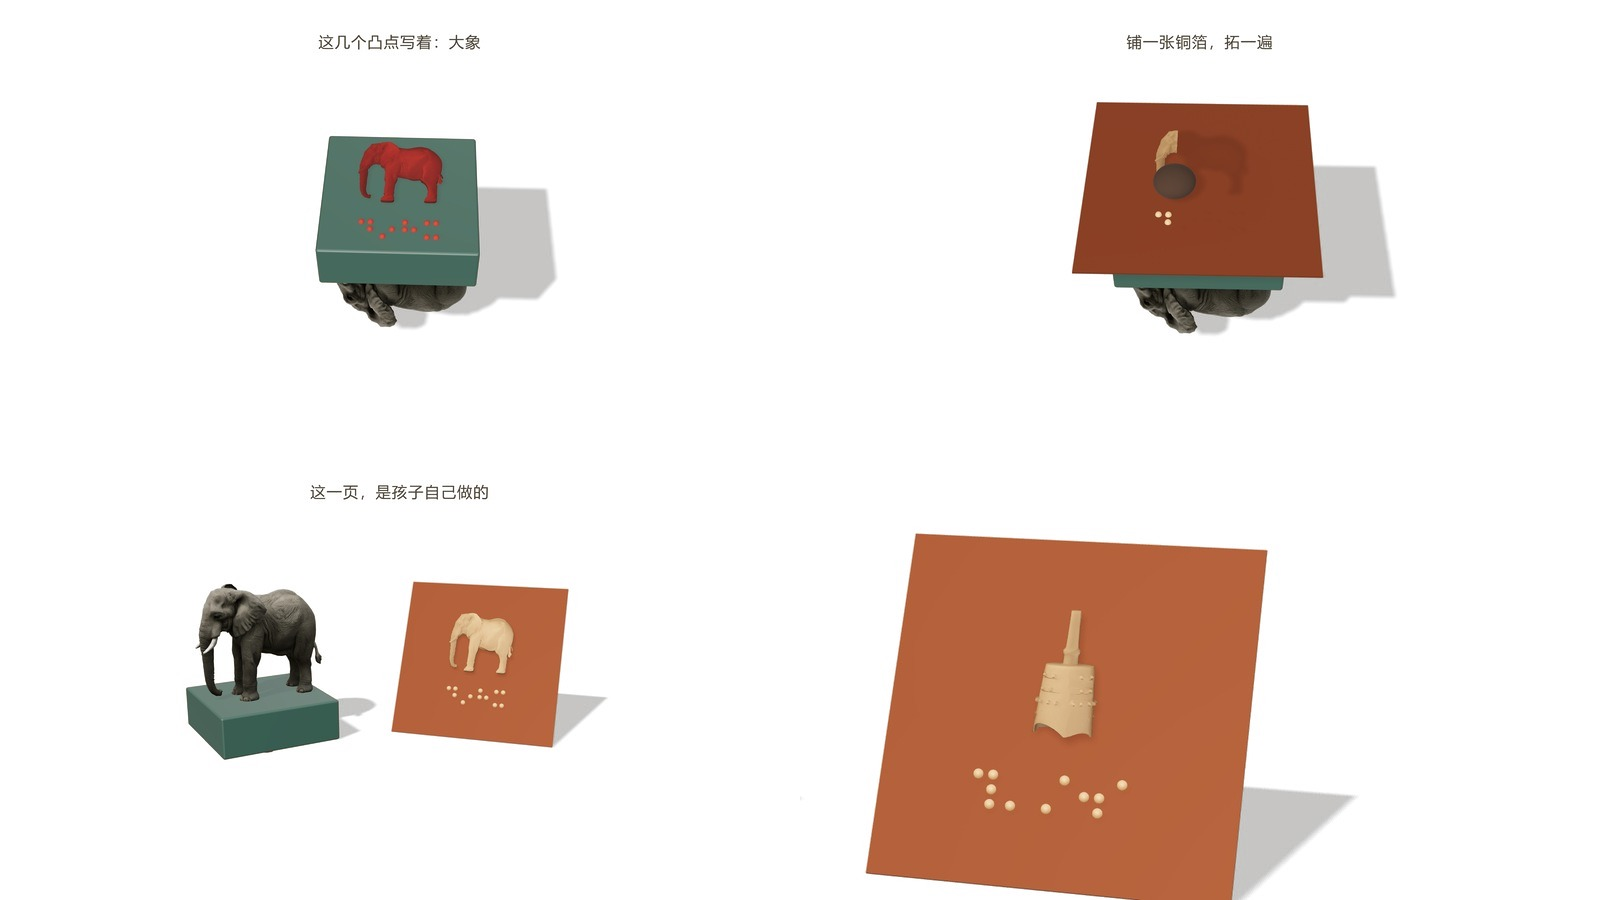
\includegraphics[width=\linewidth]{keyframes.jpg}
\end{minipage}\hfill
\begin{minipage}[c]{0.47\linewidth}
\captionsetup{justification=raggedright,singlelinecheck=false}
\caption{12 秒动画的关键帧。\newline 左上：翻过来，“这几个凸点写着：大象”；\newline 右上：铺一张铜箔，深色圆头工具抹过，浮雕随接触逐步显出；\newline 左下：立起这一页，“这一页，是孩子自己做的”；\newline 右下：甬钟拓片近景，钟身上的成排枚和下缘凹口都看得清。}
\label{fig:keyframes}
\end{minipage}
\end{figure}

\subsection{八枚印的三联图}
\begin{figure}[H]
\centering
\newcommand\cell[2]{\begin{minipage}[t]{0.325\linewidth}\centering\includegraphics[width=\linewidth]{tripc_#1.png}\\[-1pt]{\scriptsize\sffamily\color{stone}#2}\end{minipage}}
\cell{elephant}{\textbf{大象} · 太大 · 身长约 6 米}\hfill\cell{blue_whale}{\textbf{蓝鲸} · 太深 · 身长约 25 米}\hfill\cell{trex}{\textbf{霸王龙} · 已经灭绝 · 身长约 12 米}\\[4pt]
\cell{shark}{\textbf{大白鲨} · 太危险 · 身长约 4.5 米}\hfill\cell{ant}{\textbf{蚂蚁} · 太小 · 身长不到 1 厘米}\hfill\cell{saturn}{\textbf{土星} · 太远 · 光环宽约 27 万公里}\\[4pt]
\cell{volcano}{\textbf{火山} · 太烫 · 高几千米}\hspace{0.0125\linewidth}\cell{yongzhong}{\textbf{甬钟} · 隔着展柜 · 高约 45 厘米}
\caption{八枚印的三联图：每张从左到右依次是印钮、印面（盲文 + 轮廓浮雕）、拓出来的一页。}
\label{fig:triptychs}
\end{figure}

\subsection{演示视频}
\texttt{盼盼法式小面包-万物印-演示视频.mp4}：106 秒，1920$\times$1080，无旁白，只有文字字幕和配乐；配乐由我们自己的脚本合成，没有使用第三方音频。

\begin{note}[colback=white!60!cream]
{\sffamily\bfseries\color{stone}结构}\quad
闭眼开场（黑底三句）$\to$ 七枚“摸不到”快切 $\to$ 标题 $\to$ 三联图 $\to$ 大象：摸、翻面、拓印、成页 $\to$ \textbf{造印机实机录屏}：输入“我想摸摸长颈鹿” $\to$ Lux3D 文生 3D $\to$ 落桌、翻面、拓印 $\to$ 上传大都会艺术博物馆 CC0 青铜钟照片（DP155212，春秋） $\to$ Lux3D 图生 3D $\to$ 双龙钟钮的印 $\to$ 材质重绘三材 $\to$ 十枚印合影（含两枚现场新铸） $\to$ 片尾。
\end{note}

画面全部来自真实运行的网页：造印机部分用 Playwright 驱动页面，通过 Chrome DevTools 的屏幕流录制；展示部分是 \texttt{seal.html} 的逐帧渲染。等待生成的片段在画面上加速播放，并标出实际等待时间。制作脚本和步骤在仓库 \path{web/tools/video/}（README.md）。

\begin{figure}[H]
\centering
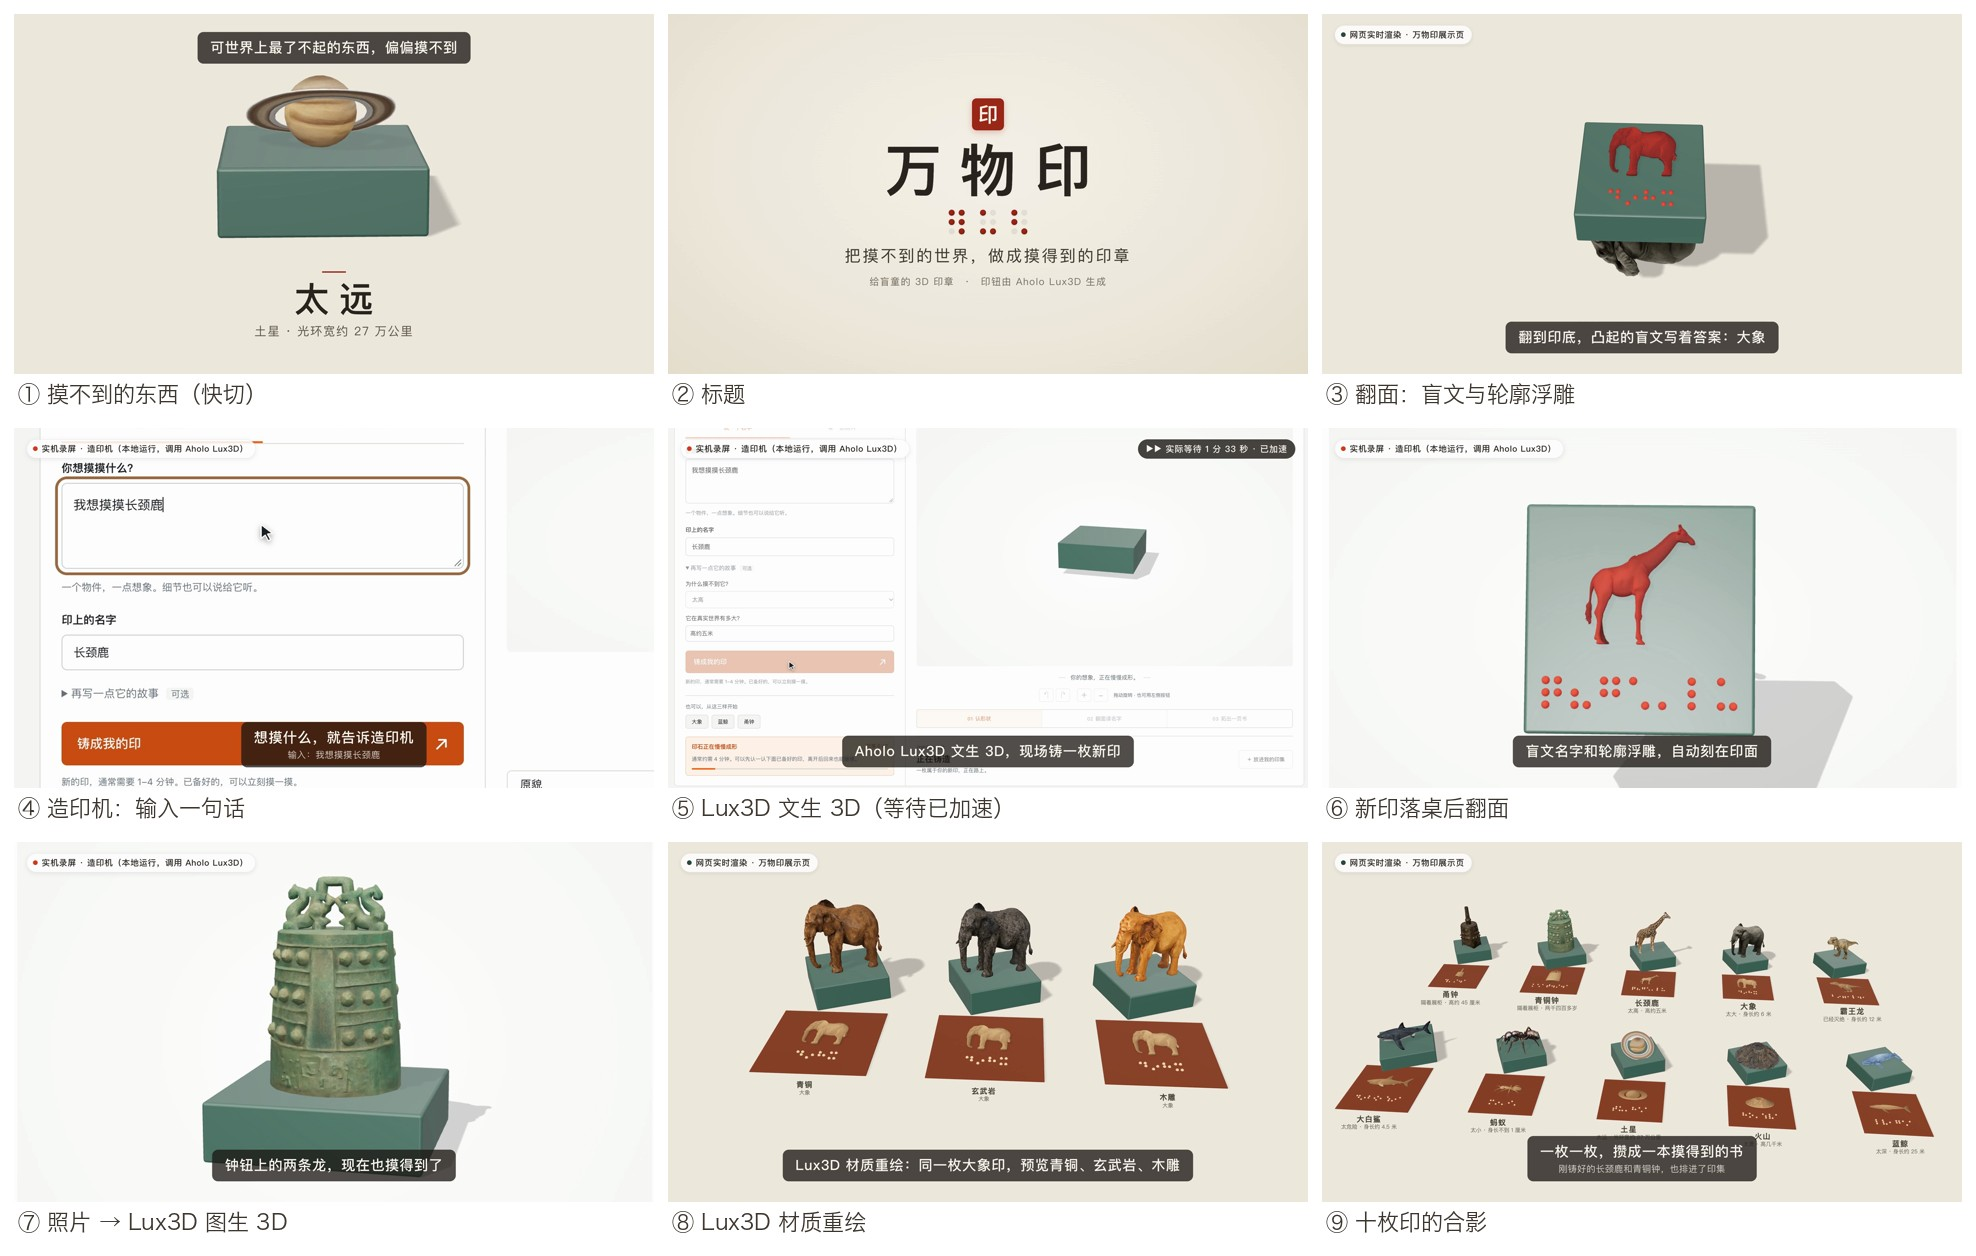
\includegraphics[width=\linewidth]{video_frames.jpg}
\caption{演示视频关键帧：①摸不到的东西；②标题；③翻面读盲文；④造印机输入一句话；⑤Lux3D 文生 3D（等待已加速）；⑥新印落桌后翻面；⑦照片 $\to$ Lux3D 图生 3D；⑧材质重绘；⑨十枚印合影。}
\label{fig:video}
\end{figure}

\subsection{能运行的东西}
代码仓库公开在 \url{https://github.com/zicheng-yu/wanwuyin}。克隆后在 \texttt{web/} 下执行 \texttt{npm ci} 与 \texttt{npx vite -{}-port 5199}，就能在本机打开下面这些页面；在线铸造新印还需要按 README 启动本机后端并配置自己的 Lux3D 密钥。

\noindent{\small
\renewcommand{\arraystretch}{1.28}%
\begin{tabularx}{\linewidth}{@{}>{\ttfamily}l X@{}}
\toprule
\normalfont\sffamily 页面 & \sffamily 内容 \\
\midrule
maker.html & 造印工作台：文字 / 照片造印、翻面拓印、换印材、收藏、离线体验 \\
seal.html?seal=elephant & 单枚印三联图（印钮 / 印面 / 拓片），可拖动视角；\texttt{seal=} 可换成其他七枚 \\
seal.html?view=set & 八枚合影 \\
seal.html?view=set\&materials=1 & 同一枚大象印的青铜、玄武岩、木雕三材合影 \\
seal.html?view=anim\&seal=elephant & 12 秒动画：摸 $\to$ 翻面 $\to$ 拓印 $\to$ 成页 \\
\bottomrule
\end{tabularx}}

此外，仓库 Release 里的 \texttt{snapshot-2026-11-11} 保存了 Lux3D 原始输出与渲染快照；38.9 秒的无声概念片在 \path{docs/media/wanwuyin_concept.mp4}。

% =====================================================================
\section{为盲童设计的细节}\label{sec:blind}

\begin{itemize}[leftmargin=1.4em,itemsep=4pt]
  \item \textbf{国家通用盲文，常见尺寸。}名字由 liblouis 的 \texttt{zhcn-cbs.ctb} 表转写为国家通用盲文。数字模型里点距 2.5 毫米、方距 6 毫米、点径约 1.7 毫米、点高约 0.95 毫米，取常见盲文尺寸；名字里的数字写成汉字（数字盲文规则待确认）。
  \item \textbf{凸起、正向。}印面上的盲文本身就是正向凸点，翻过来直接摸读；拓片同样凸起、正向（图 \ref{fig:rubbing}）。
  \item \textbf{先摸后验，独立完成。}印钮上不放文字，答案只在印底；孩子不需要等明眼人揭晓，自己就能核对。
  \item \textbf{为手选角度。}每枚印单独选浮雕的压平角度，保证手能区分的特征留在印面上：土星的环孔、蓝鲸的尾鳍、蚂蚁的六条腿、火山口（第 \ref{sec:iter} 小节）。浮雕高约 2 毫米。
  \item \textbf{握在手心。}印面边长约 4.4 厘米起，按盲文长度加宽（最长的“大白鲨”约 5.4 厘米），印钮最高约 5.4 厘米。
  \item \textbf{真实尺寸。}每枚印都带一句真实尺寸（“身长约 25 米”），方便老师把手里的小印和真实世界的大小联系起来讲。
  \item \textbf{网页可以只用键盘操作。}按钮都有可访问名称，生成状态通过状态区域更新播报；尊重“减少动态效果”偏好，动作直接到达对应状态；有浅色 / 深色主题。VoiceOver 的实际播报还需要在设备上复核。
  \item \textbf{没有网络也能玩。}“准备离线体验”会缓存页面和大象、蓝鲸、甬钟三枚印的模型，断网刷新后仍能完整地认形状、翻面、拓印、收藏，适合网络不好的教室。
\end{itemize}

% =====================================================================
\section{局限与下一步}\label{sec:next}

\subsection{局限}
\begin{enumerate}[leftmargin=1.6em,itemsep=3pt]
  \item \textbf{还没有打印实物。}报告和视频里的印都是数字渲染；盲文点和浮雕在实物上能不能摸清，要试印后才知道。
  \item \textbf{还没有和盲童、特教老师一起测试。}玩法来自我们的设想，尚未经过真实使用的检验。
  \item \textbf{盲文没有经过专业校对。}目前是 liblouis 自动转写，数字的盲文规则也待确认。
  \item \textbf{Lux3D 的结果需要人把关。}第一版蚂蚁不适合数腿；尺度不可靠（霸王龙生成为 0.5 米）；多视图重建会把棱角抹圆。
  \item \textbf{在线铸造依赖本机后端。}密钥不进前端，所以现场生成新印需要运行后端；只体验已备好的印则不需要。
\end{enumerate}

\subsection{下一步}
\begin{enumerate}[leftmargin=1.6em,itemsep=3pt]
  \item \textbf{两件式可打印印章。}印钮和带印面的印身分开打印再拼合：印面朝上平放打印，盲文点更清楚；印钮可以单独选材料。
  \item \textbf{试印与校对。}请盲文老师校对八枚印的盲文，用实物调整点高、点距和浮雕高度。
  \item \textbf{走进特教学校试用。}和老师一起观察孩子怎么摸、怎么猜、怎么拓，再改玩法。
  \item \textbf{扩充印集。}候补有月球（太远，用几个宽浅的环形山体现手感）和三叶虫化石（已经灭绝，靠分节背甲辨形）；也可以把课本插图直接变成印。
  \item \textbf{彩蛋：万物有声。}把「万物有声」接回来，敲一敲甬钟印，听到按它的 Lux3D 模型算出来的声音。
\end{enumerate}

% =====================================================================
\section{素材与工具声明}\label{sec:credits}
\begin{itemize}[itemsep=3pt]
  \item \textbf{3D 模型：}全部印钮由 Aholo Lux3D 生成，任务号见第 \ref{sec:lux} 节。
  \item \textbf{图片素材：}大都会艺术博物馆开放获取（The Met Open Access，CC0）照片：战国青铜甬钟 DP154556（甬钟印钮、四视图与多视图重建的输入），春秋青铜钟 DP155212（演示视频中现场图生 3D 的输入）。材质重绘的参考图来自项目留存的馆藏素材（青铜锈、玄武岩石臼、木雕根付，木雕藏品编号 MET 10.211.2034）。
  \item \textbf{软件：}Aholo Lux3D OpenAPI；three.js、Vite（网页与渲染）；liblouis（国家通用盲文转写）；trimesh（朝向计算）；glTF-Transform 与 meshoptimizer（模型压缩）；playwright-core 与 FFmpeg（截图与录制）；Python 标准库与 SQLite（造印机后端）。
  \item \textbf{现场生成：}演示视频里的长颈鹿印和青铜钟印，是录制时用造印机现场调用 Lux3D 生成的，没有人工修改模型。
  \item \textbf{音乐：}演示视频的配乐由我们自己的合成脚本（\path{web/tools/video/music.py}）生成，没有使用第三方音频。
  \item \textbf{字体：}视频文字使用系统自带的苹方（PingFang SC）；本报告使用 macOS 系统自带字体排版。
  \item \textbf{AI 辅助：}开发中使用了 AI 编程助手（Claude Code、OpenAI Codex、Cursor）辅助编写代码、文档和本报告；方向与取舍由团队决定和确认。
  \item \textbf{图片说明：}报告中的印章、拓片、动画画面均为数字渲染，不是实物照片。
\end{itemize}

% =====================================================================
\section{团队与链接}\label{sec:links}
\begin{note}[colback=white!60!cream]
\renewcommand{\arraystretch}{1.45}
\begin{tabularx}{\linewidth}{@{}>{\sffamily\bfseries\leavevmode\color{stone}}p{2.6cm}X@{}}
团队 & \team \\
代码仓库 & \url{https://github.com/zicheng-yu/wanwuyin}（公开；README 有本机运行命令） \\
演示视频 & \texttt{盼盼法式小面包-万物印-演示视频.mp4}（随作品提交；无旁白，字幕 + 背景音乐，网页实录） \\
概念片 & 仓库内 \path{docs/media/wanwuyin_concept.mp4}（38.9 秒，无声） \\
视频制作脚本 & 仓库 \path{web/tools/video/}（README.md 有完整步骤） \\
生成物快照 & 仓库 Release \texttt{snapshot-2026-11-11}（Lux3D 原始输出、渲染） \\
\end{tabularx}
\end{note}

\subsection*{结语}
万物印想做的事很小：让看不见的孩子把大象、蓝鲸、土星这些一辈子摸不到的东西握在手里，自己猜，自己翻过来核对，再自己拓出一页。Lux3D 让“想摸什么就造什么”第一次变得可行。它现在还只是数字原型；接下来我们最想做的，是把第一批印打印出来，请盲文老师校对，再交到孩子和老师手里，听他们说哪里好、哪里不对。

\medskip
{\centering\kai\Large\color{stone} 摸不到的世界，一枚一枚握在手里。\par}

\end{document}
